\documentclass[table]{beamer}
%[]中可以使用draft、handout、screen、transparency、trancompress、compress等参数

%指定beamer的模式与主题
\mode<presentation>
{
  \usetheme{Madrid}
%\usetheme{Boadilla}
%\usecolortheme{default}
%\usecolortheme{orchid}
%\usecolortheme{whale}
%\usefonttheme{professionalfonts}
}

%\usetheme{Madrid}
%这里还可以选择别的主题:Bergen, Boadilla, Madrid, AnnArbor, CambridgeUS, Pittsburgh, Rochester, Warsaw, ...
%有导航栏的Antibes, JuanLesPins, Montpellier, ...
%有内容的Berkeley, PaloAlto, Goettingen, Marburg, Hannover, ...
%有最小导航栏的Berlin, Ilmenau, Dresden, Darmstadt, Frankfurt, Singapore, Szeged, ...
%有章和节表单的Copenhagen, Luebeck, Malmoe, Warsaw, ...

%\usecolortheme{default}
%设置内部颜色主题(这些主题一般改变block里的颜色);这个主题一般选择动物来命名
%这里还可以选择别的颜色主题,如默认的和有特别目的的颜色主题default,structure,sidebartab,全颜色主题albatross,beetle,crane,dove,fly,seagull,wolverine,beaver

%\usecolortheme{orchid}
%设置外部颜色主题(这些主题一般改变title里的颜色);这个主题一般选择植物来命名
%这里还可以选择别的颜色主题,如默认的和有特别目的的颜色主题lily,orchid,rose

%\usecolortheme{whale}
%设置字体主题;这个主题一般选择海洋动物来命名
%这里还可以选择别的颜色主题,如默认的和有特别目的的颜色主题whale,seahorse,dolphin

%\usefonttheme{professionalfonts}
%类似的还可以定义structurebold,structuresmallcapsserif,professionalfonts


% 控制 beamer 的风格,可以根据自己的爱好修改
%\usepackage{beamerthemesplit} %使用 split 风格
%\usepackage{beamerthemeshadow} %使用 shadow 风格
%\usepackage[width=2cm,dark,tab]{beamerthemesidebar}

%插入音标
\usepackage{tipa}
\AtBeginDocument{
  \renewcommand\textipa{\fontencoding{T3}\selectfont}
}
\AtBeginDocument{
  \renewcommand\textipa[2][r]{{\fontfamily{cm#1}\tipaencoding #2}}
}
\renewenvironment{IPA}[1][r]
 {\fontfamily{cm#1}\tipaencoding}
 {}

% 设定英文字体
%\usepackage{fontspec}
\usepackage[no-math]{fontspec}
\setmainfont{Times New Roman}
\setsansfont{Arial}
\setmonofont{Courier New}

% 设定中文字体
\usepackage[BoldFont,SlantFont,CJKchecksingle,CJKnumber]{xeCJK}
%\setCJKmainfont[BoldFont={Adobe Heiti Std},ItalicFont={Adobe Kaiti Std}]{Adobe Song Std}
\setCJKmainfont[BoldFont={Adobe Heiti Std},ItalicFont={Adobe Kaiti Std}]{WenQuanYi Micro Hei}
\setCJKsansfont{Adobe Heiti Std}
\setCJKmonofont{Adobe Fangsong Std}
\punctstyle{hangmobanjiao}

\defaultfontfeatures{Mapping=tex-text}
\usepackage{xunicode}
\usepackage{xltxtra}

\XeTeXlinebreaklocale "zh"
\XeTeXlinebreakskip = 0pt plus 1pt minus 0.1pt

\usepackage{setspace}
\usepackage{colortbl,xcolor}
\usepackage{hyperref}
%\hypersetup{xetex,bookmarksnumbered=true,bookmarksopen=true,pdfborder=1,breaklinks,colorlinks,linkcolor=blue,filecolor=black,urlcolor=cyan,citecolor=green}
\hypersetup{xetex,bookmarksnumbered=true,bookmarksopen=true,pdfborder=1,breaklinks,colorlinks,linkcolor=cyan,filecolor=black,urlcolor=blue,citecolor=green}

% 插入图片
\usepackage{graphicx}
\graphicspath{{figures/}}
% 图文混排
\usepackage{picins}
\usepackage{floatflt}

% 可能用到的包
\usepackage{amsmath,amssymb}
%插入多媒体
%\usepackage{media9}
%\usepackage{movie15}
\usepackage{multimedia}
\usepackage{multicol}
\usepackage{multirow}

% 定义一些自选的模板,包括背景、图标、导航条和页脚等,修改要慎重
% 设置背景渐变由10%的红变成10%的结构颜色
%\beamertemplateshadingbackground{red!10}{structure!10}
%\beamertemplatesolidbackgroundcolor{white!90!blue}
% 使所有隐藏的文本完全透明、动态,而且动态的范围很小
\beamertemplatetransparentcovereddynamic
% 使itemize环境中变成小球,这是一种视觉效果
\beamertemplateballitem
% 为所有已编号的部分设置一个章节目录,并且编号显示成小球
\beamertemplatenumberedballsectiontoc
% 将每一页的要素的要素名设成加粗字体
\beamertemplateboldpartpage

% item逐步显示时,使已经出现的item、正在显示的item、将要出现的item呈现不同颜色
\def\hilite<#1>{
 \temporal<#1>{\color{gray}}{\color{blue}}
    {\color{blue!25}}
}

\renewcommand{\today}{\number\year 年 \number\month 月 \number\day 日}

%五角星
\usepackage{MnSymbol}

%去除图表标题中的figure等
\usepackage{caption}
\captionsetup{labelformat=empty,labelsep=none}

\usepackage{tabu}
\usepackage{multirow}
%表格自动换行
\usepackage{tabularx} 

% 千分号
%\usepackage{textcomp}

%罗马数字
\makeatletter
\newcommand{\rmnum}[1]{\romannumeral #1}
\newcommand{\Rmnum}[1]{\expandafter\@slowromancap\romannumeral #1@}
\makeatother

%分栏
\usepackage{multicol}

%\usepackage{enumitem}
%\usepackage{enumerate}

%键盘
\usepackage{keystroke}

%插入源代码
\usepackage{listings}
\lstset{
  language=bash,                  % 程序语言名称:TeX, Perl, R, sh, bash, Awk
  basicstyle=\normalsize\tt,      %\tt指monospace字体族,程序源代码使用此族字体表示更加美观
  numbers=left,                   % 行号位置(左侧)
  numberstyle=\small,             % 行号字体的字号
  stepnumber=1,                   % 行号的显示步长
  numbersep=5pt,                  % 行号与代码间距
  backgroundcolor=\color{white},  % 背景色;需要 \usepackage{color}
  showspaces=false,               % 不显示空格
  showstringspaces=false,         % 不显示代码字符串中的空格标记
  showtabs=false,                 % 不显示 TAB
  tabsize=4, 
  frame=shadowbox,                % 把代码用带有阴影的框圈起来
  captionpos=b,                   % 标题位置
  breaklines=true,                % 对过长的代码自动断行
  breakatwhitespace=false,        % 断行只在空格处
  extendedchars=false,            % 解决代码跨页时,章节标题,页眉等汉字不显示的问题
  %escapeinside={\%*}{*},         % 跳脱字符,添加注释,暂时离开 listings 
  %escapeinside=``,
  commentstyle=\color{red!50!green!50!blue!50}\tt,  %浅灰色的注释
  rulesepcolor=\color{red!20!green!20!blue!20},     %代码块边框为淡青色
  keywordstyle=\color{blue!70}\bfseries\tt,         %代码关键字的颜色为蓝色,粗体
  identifierstyle=\tt,
  stringstyle=\tt,                % 代码字符串的特殊格式
  keepspaces=true,
  breakindent=1em,
  %breakindent=22pt,
  %breakindent=4em,
  breakautoindent=true,
  flexiblecolumns=true,
  aboveskip=1em,                  %代码块边框
  xleftmargin=2em,
  xrightmargin=2em
}

%\setbeamercolor{alerted text}{fg=magenta}
\setbeamercolor{bgcolor}{fg=yellow,bg=cyan}
%\setbeamercolor{itemize/enumerate body}{fg=green}

\begin{document}

%\includeonlyframes{current}

\logo{
\includegraphics[height=0.08\textwidth]{tijmu.png}}

% 在每个Section前都会加入的Frame
\AtBeginSection[]
{
  \begin{frame}<beamer>
    %\frametitle{Outline}
    \frametitle{教学提纲}
    \setcounter{tocdepth}{3}
    \begin{multicols}{2}
      \tableofcontents[currentsection,currentsubsection]
      %\tableofcontents[currentsection]
    \end{multicols}
  \end{frame}
}
% 在每个Subsection前都会加入的Frame
\AtBeginSubsection[]
{
  \begin{frame}<beamer>
%%\begin{frame}<handout:0>
%% handout:0 表示只在手稿中出现
    \frametitle{教学提纲}
    \setcounter{tocdepth}{3}
    \begin{multicols}{2}
    \tableofcontents[currentsection,currentsubsection]
    \end{multicols}
%% 显示在目录中加亮的当前章节
  \end{frame}
}

% 为当前幻灯片设置背景
%{
%\usebackgroundtemplate{
%\vbox to \paperheight{\vfil\hbox to
%\paperwidth{\hfil
\includegraphics[width=2in]{tijmu_charcoal.png}\hfil}\vfil}
%}
\begin{frame}[plain]
  \begin{center}
    {\Huge Linux系统概论\\}
    \vspace{1cm}
    {\LARGE 天津医科大学\\}
    %\vspace{0.2cm}
    {\LARGE 生物医学工程与技术学院\\}
    \vspace{1cm}
    {\large 2017-2018学年下学期(春)\\ 2016级生信班}
  \end{center}
\end{frame}
%}



%\includeonlyframes{current}

\title[shell编程]{第八章\quad shell编程}
\author[Yixf]{伊现富(Yi Xianfu)}
\institute[TIJMU]{天津医科大学(TIJMU)\\ 生物医学工程与技术学院}
\date{2016年4月}


\begin{frame}
  \titlepage
\end{frame}

\begin{frame}[plain,label=current]
  \frametitle{教学提纲}
  \setcounter{tocdepth}{3}
  \begin{multicols}{2}
    \tableofcontents
  \end{multicols}
\end{frame}


\section{引言}
\begin{frame}
  \frametitle{引言 | shell的职责}
  \begin{figure}
    \centering
    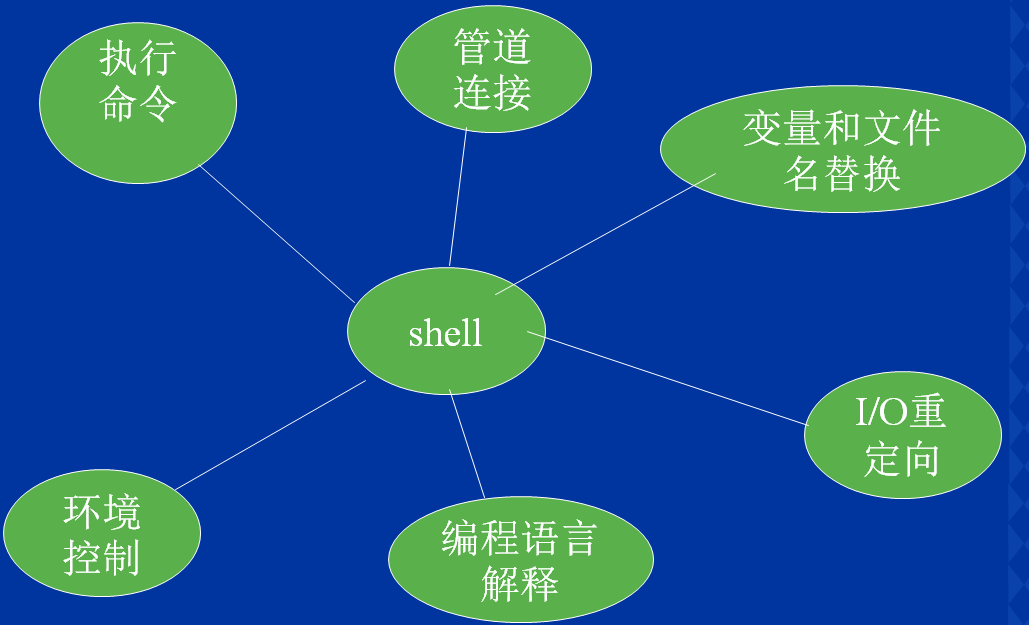
\includegraphics[width=10cm]{c8.shell.function.01.png}
  \end{figure}
\end{frame}

\begin{frame}
  \frametitle{引言 | shell脚本}
  \begin{block}{shell脚本}
    shell程序通常称为脚本(script),是存储在单个文件中的一系列系统命令。\\
    每次调用shell脚本时,其中的命令就会自动地依次执行。\\
    shell脚本可用于很多方面,特别是用于系统管理。通过shell脚本,可以利用少数的简单脚本自动完成大量的工作。\\
    shell脚本实质上是一组按顺序执行的命令。
  \end{block}
  \begin{figure}
    \centering
    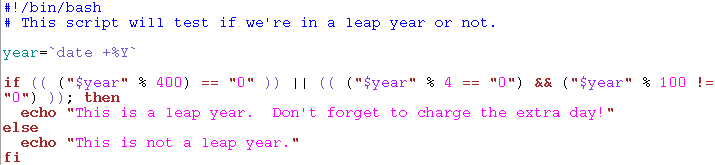
\includegraphics[width=7cm,height=2cm]{c8.shell.example.01.png}
    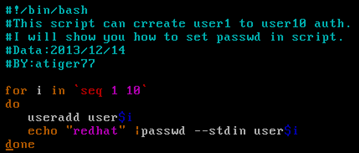
\includegraphics[width=5cm]{c8.shell.example.02.png}
  \end{figure}
\end{frame}

\begin{frame}
  \frametitle{引言 | shell脚本}
  Scripts are a sequence of statements and commands stored in a file that can be executed by a shell. The most commonly used shell in Linux is \textbf{bash}.
\end{frame}

\begin{frame}
  \frametitle{引言 | shell脚本 | 命令}
  \begin{columns}
    \column{0.5\textwidth}
  Shell scripts are used to execute sequences of commands and other types of statements. Commands can be divided into the following categories:
  \begin{itemize}
    \item Compiled applications
    \item Built-in \textbf{bash} commands
    \item Other scripts
  \end{itemize}
  \column{0.5\textwidth}
    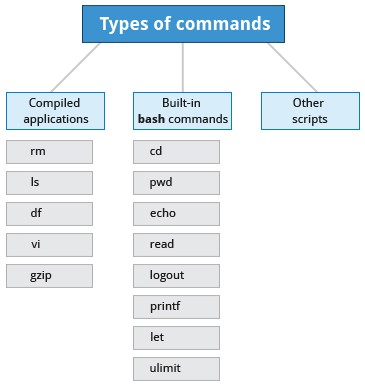
\includegraphics[width=\textwidth]{c8.command.type.jpg}
  \end{columns}
\end{frame}

\begin{frame}[fragile]
  \frametitle{引言 | shell脚本 | 命令}
  Compiled applications are binary executable files that you can find on
  the filesystem. The shell script always has access to compiled
  applications such as \textbf{rm}, \textbf{ls} , \textbf{df} ,
  \textbf{vi} , and \textbf{gzip}.\\
  \vspace{0.3cm}
  \textbf{bash} has many \textbf{built-in} commands which can only be used to display the output within a terminal shell or shell script. Sometimes these commands have the same name as executable programs on the system, such as \textbf{echo} which can lead to subtle problems. \textbf{bash} built-in commands include and \verb|cd|, \verb|pwd|, \verb|echo|, \verb|read|, \verb|logout|, \verb|printf|, \verb|let|, and \verb|ulimit|.\\
  \vspace{0.3cm}
  A complete list of \textbf{bash} built-in commands can be found in the \textbf{bash man} page, or by simply typing \verb|help|.
\end{frame}

\begin{frame}
  \frametitle{引言 | shell脚本 | 用途}
  \begin{figure}
    \centering
    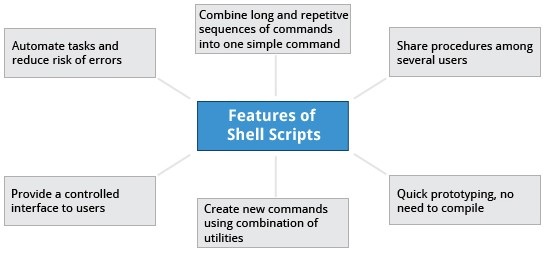
\includegraphics[width=12cm]{c8.shell.script.feature.jpg}
  \end{figure}
\end{frame}

\begin{frame}
  \frametitle{引言 | shell脚本 | 实例}
  \begin{figure}
    \centering
    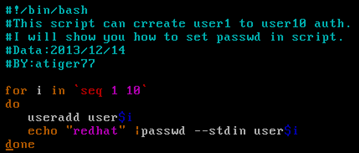
\includegraphics[width=6cm]{c8.shell.example.02.png}\quad
    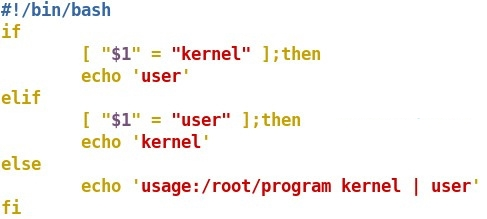
\includegraphics[width=5.5cm]{c8.shell.example.03.jpg}\\
    \vspace{0.5cm}
    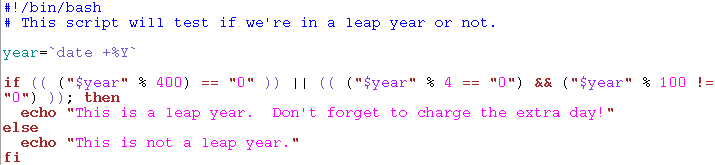
\includegraphics[width=11cm]{c8.shell.example.01.png}
  \end{figure}
\end{frame}

\section{编程起步}
\subsection{脚本结构与运行}
\begin{frame}[fragile]
  \frametitle{引言 | shell脚本 | 实例}
\begin{lstlisting}
#!/bin/bash

#This is to show what a example looks like.

echo "Our first example!"
echo # This inserts an empty line in output.
echo "We are currently in the following directory:"
pwd
echo
echo "This directory contains the following files:"
ls
\end{lstlisting}
\end{frame}

\begin{frame}[fragile]
  \frametitle{编程起步 | \alert{脚本结构}}
  \begin{block}{shell脚本的结构}
    \begin{itemize}
      \item \#!调用shell(指定执行脚本的shell)。
      \item \#进行注释。
      \item 命令和控制结构。
      \item shell命令,可以按照分号分隔,也可以按照换行符分隔。
      \item 如果想在一行中写入多个命令,可以通过分号(;)分隔。
    \end{itemize}
  \end{block}
  \pause
  \begin{block}{创建shell脚本的步骤}
    \begin{enumerate}
      \item 创建一个包含命令和控制结构的文件。\verb|vim script.sh|
      \item 修改文件的权限使它可执行。\verb|chmod u+x script.sh|
      \item 运行文件。\verb|./script.sh|或 \verb|sh script.sh|(不需要可执行权限)
    \end{enumerate}
  \end{block}
\end{frame}

\begin{frame}
  \frametitle{编程起步 | 脚本运行}
  \begin{figure}
    \centering
    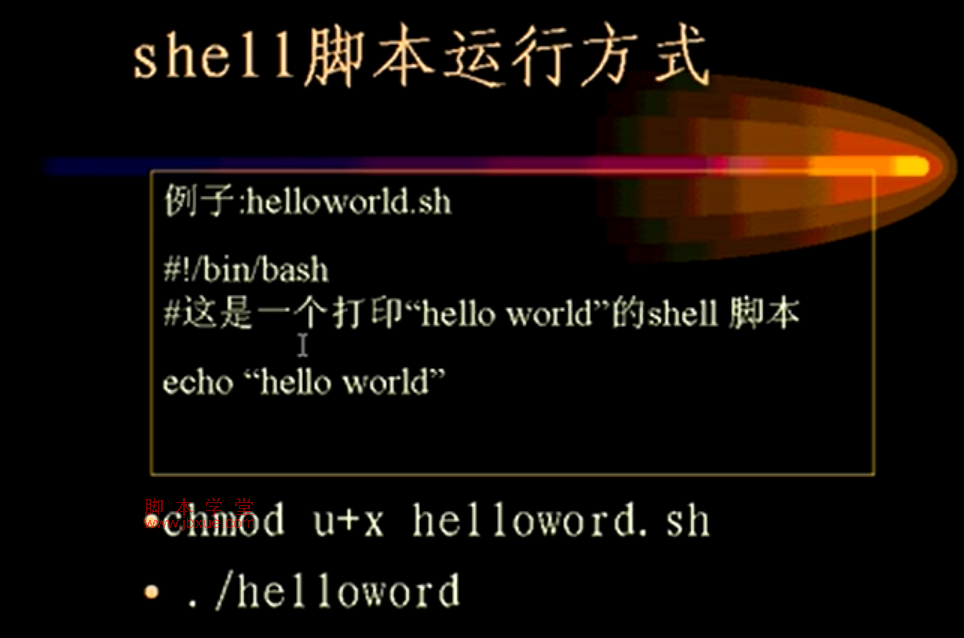
\includegraphics[width=10cm]{c8.shell.shebang.01.png}
  \end{figure}
\end{frame}

\begin{frame}
  \frametitle{编程起步 | 脚本运行}
  \begin{figure}
    \centering
    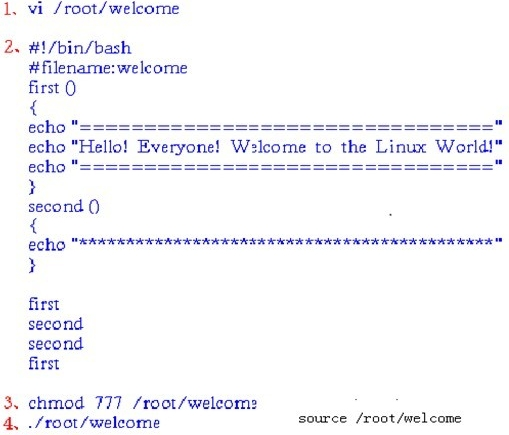
\includegraphics[width=9cm]{c8.shell.shebang.02.jpg}
  \end{figure}
\end{frame}

\subsection{调用shell}
\begin{frame}[fragile]
  \frametitle{编程起步 | \alert{调用shell}}
  \begin{itemize}
    \item 在向脚本中添加任何其他内容之前,用户需要告诉系统将要启动一个shell脚本。
    \item 使用shebang结构,如:\verb|#!/bin/bash|告诉系统接下来的命令由bash shell执行。
    \item 要创建一个脚本,用户应该首先添加shebang行,然后添加命令。
    \item shebang是因为 \verb|#|称为hash,\verb|!|称为bang。
  \end{itemize}
\end{frame}

\begin{frame}[fragile]
  \frametitle{编程起步 | 调用shell | 种类}
  \begin{columns}
    \column{0.5\textwidth}
\begin{lstlisting}
$cat /etc/shells
# /etc/shells: valid login shells
/bin/sh
/bin/dash
/bin/bash
/bin/rbash
/bin/tcsh
/usr/bin/tcsh
/usr/bin/tmux
/bin/ksh93
/usr/bin/screen
\end{lstlisting}
    \column{0.5\textwidth}
    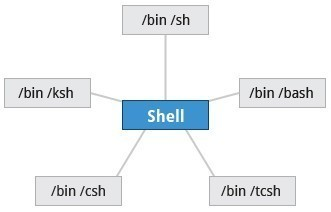
\includegraphics[width=\textwidth]{c8.shells.jpg}
  \end{columns}
\end{frame}

\begin{frame}[fragile]
  \frametitle{编程起步 | 调用shell | 实例}
\begin{lstlisting}
#!/bin/bash

# /home/yixf/dirinfo
# 2014年 06月 24日
# A really stupid script to give some basic info about the current directory

pwd
ls
\end{lstlisting}
\end{frame}

%\subsection{脚本注释}
\subsection{特殊字符}
\begin{frame}
  \frametitle{编程起步 | \alert{特殊字符}}
  \begin{figure}
    \centering
    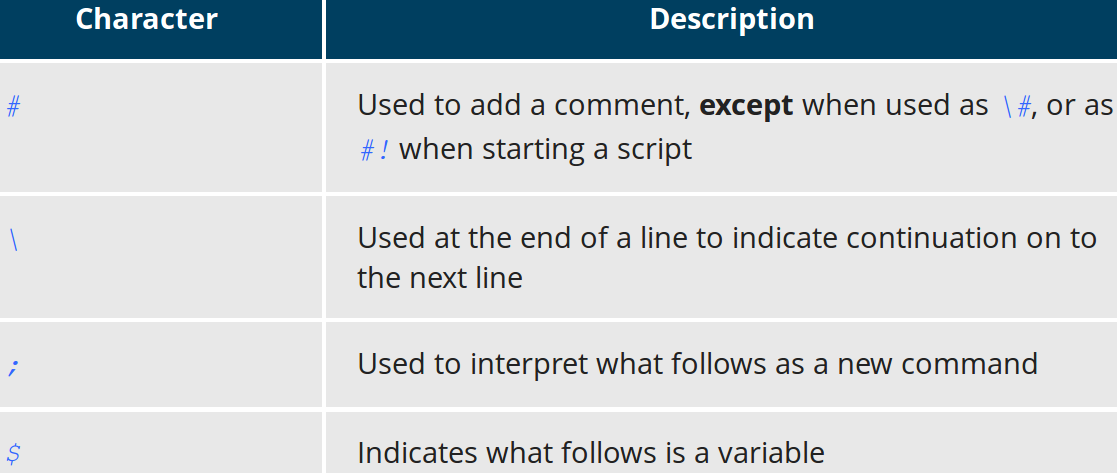
\includegraphics[width=11cm]{c8.comment.10.png}
  \end{figure}
\end{frame}

\begin{frame}
  \frametitle{编程起步 | 特殊字符 | 脚本注释 | 注释简介}
  好的注释对好的程序而言非常关键:为什么编写它、脚本中各部分的作用、如何使用脚本、……\\
  shell脚本是独立的文档,因此注释它们的最简单也是最好的方法是使用脚本自己的注释。
\end{frame}

\begin{frame}[fragile]
  \frametitle{编程起步 | 特殊字符 | 脚本注释 | \alert{注释方法}}
  \begin{block}{注释方法}
    \begin{itemize}
      \item 注释行以散列符号(\verb|#|)开头,在 \verb|#|之后出现的所有内容都认为是注释,不解释为命令。
      \item 占用多行的注释在每行的开头都有一个 \verb|#|。
      \item 可以在一行的中间插入 \verb|#|,\verb|#|右边的所有内容都将看作注释。
    \end{itemize}
  \end{block}
  \pause
\begin{lstlisting}
# Here is a comment that
# spans multipe lines.
command # This is comment explaining the cmd
\end{lstlisting}
\end{frame}

\begin{frame}
  \frametitle{编程起步 | 特殊字符 | 脚本注释 | 经验之谈}
  \begin{itemize}
    \item 在脚本的顶部放置一些基本信息。\\ \qquad 包括:脚本的名称、日期、脚本的总体作用、命令行参数的正确语法、脚本的不同寻常之处、……
    \item 保存脚本的修改日志。\\ \qquad 将每个修改添加到修改日志的顶部。
    \item 注释脚本的每个部分。\\ \qquad 说明每个部分的作用或目的。
    \item 识别必须由用户添加的数据。\\ \qquad 解释需要添加的信息以及该信息需要的格式。
  \end{itemize}
\end{frame}

\begin{frame}[fragile]
  \frametitle{编程起步 | 特殊字符 | Splitting Long Commands Over Multiple Lines}
  Users sometimes need to combine several commands and statements and even conditionally execute them based on the behaviour of operators used in between them. This method is called \textbf{chaining of commands}.\\
  \vspace{0.2cm}
  The \textbf{concatenation operator} (\verb|\|) is used to concatenate large commands over several lines in the shell.\\
  \vspace{0.2cm}
  The command is divided into multiple lines to make it look readable and easier to understand. The \verb|\| operator at the end of each line combines the commands from multiple lines and executes it as one single command.
  \begin{figure}
    \centering
    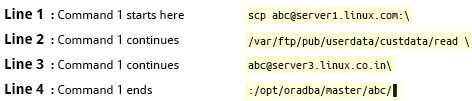
\includegraphics[width=11cm]{c8.chain.jpg}
  \end{figure}
\end{frame}

\begin{frame}[fragile]
  \frametitle{编程起步 | 特殊字符 | Putting Multiple Commands on a Single Line}
  Sometimes you may want to group multiple commands on a single line. The \verb|;| (semicolon) character is used to separate these commands and execute them sequentially as if they had been typed on separate lines.\\
  \vspace{0.2cm}
  The three commands in the following example will all execute even if the ones preceding them fail: \verb|make; make install; make clean|\\
  \vspace{0.2cm}
  However, you may want to abort subsequent commands if one fails. You can do this using the \verb|&&| (and) operator as in: \verb|make && make install && make clean|. If the first command fails the second one will never be executed.\\
  \vspace{0.2cm}
  A final refinement is to use the \verb=||= (or) operator as in: \verb=cat file1 || cat file2 || cat file3=. In this case, you proceed until something succeeds and then you stop executing any further steps.
\end{frame}

\subsection{变量}
\begin{frame}
  \frametitle{编程起步 | 变量 | 简介}
  \begin{block}{简介}
    shell传递数据的一种方法,用来代表每个取值的符号名。
  \end{block}
  \pause
  \begin{block}{分类}
    \begin{itemize}
      \item 临时变量:shell程序内部定义的,其使用范围仅限于定义它的程序,对其它程序不可见。包括:用户自定义变量、位置变量。
      \item 永久变量:环境变量,其值不随shell脚本的执行结束而消失。
    \end{itemize}
  \end{block}
\end{frame}

\begin{frame}[fragile]
  \frametitle{编程起步 | 变量 | \alert{使用}}
  \begin{itemize}
    \item 使用赋值运算符 \verb|=|对变量进行赋值,\verb|=|两边不能有空格。
    \item 如果要给变量赋空值,可以在 \verb|=|后面跟一个换行符。
    \item 在bash shell中,默认情况下将变量视作文本字符串。
    \item 通过在变量名前加一个美元符号 \verb|$|来访问该变量的值。
    \item 如果变量名的前面有美元符号 \verb|$|,那么可以将该变量替换成一个表达式。
    \item 变量名对大小写敏感。按照惯例,Linux变量用大写字母表示。
    \item 变量名长度没有限制,由字母、数字或下划线序列组成。
    \item 变量名必须以字母或下划线开头,不能用数字。
    \item 通常情况下,变量名最好使用字符和数字,并且以数字结尾。
    \item 使用set命令列出所有的变量,使用unset命令删除变量。
  \end{itemize}
\end{frame}

\begin{frame}[fragile]
  \frametitle{编程起步 | 变量 | Introduction}
  Almost all scripts use \textbf{variables} containing a value, which can be used anywhere in the script. These variables can either be user or system defined. Many applications use such \textbf{environment variables} for supplying inputs, validation, and controlling behaviour.\\
  \vspace{0.2cm}
  Some examples of standard environment variables are \verb|HOME|, \verb|PATH|, and \verb|HOST|. When referenced, environment variables must be prefixed with the \verb|$| symbol as in \verb|$HOME|. You can view and set the value of environment variables. For example, the following command displays the value stored in the \verb|PATH| variable: \verb|echo $PATH|.\\
  \vspace{0.2cm}
  However, no prefix is required when setting or modifying the variable value. For example, the following command sets the value of the \verb|MYCOLOR| variable to blue: \verb|MYCOLOR=blue|.\\
  \vspace{0.2cm}
  You can get a list of environment variables with the \textbf{env}, \textbf{set}, or \textbf{printenv} commands.
\end{frame}

\begin{frame}[fragile]
  \frametitle{编程起步 | 变量 | Exporting}
  By default, the variables created within a script are available only to the subsequent steps of that script. Any child processes (sub-shells) do not have automatic access to the values of these variables. To make them available to child processes, they must be promoted to environment variables using the \textbf{export} statement as in: \verb|export VAR=value|, or \verb|VAR=value; export VAR|.\\
  \vspace{0.2cm}
  While child processes are allowed to modify the value of exported variables, the parent will not see any changes; exported variables are not shared, but only copied.
\end{frame}
  
\begin{frame}[fragile]
  \frametitle{编程起步 | 变量 | \alert{实例}}
\begin{lstlisting}
# 变量的赋值与访问
EDITOR="vim"
echo $EDITOR # 输出:vim

num=2
echo "this is the ${num}nd" # this is the 2nd

# 默认将变量视作文本字符串
VAR=1
VAR=$VAR+1
echo $VAR # 输出文本字符串“1+1”,而不是数字2

# 变量替换(双引号)
PERSON="Fred"
echo "Hello, $PERSON" # 输出:Hello, Fred
echo 'Hello, $PERSON' # 输出:Hello, $PERSON
\end{lstlisting}
\end{frame}

\begin{frame}[fragile]
  \frametitle{编程起步 | 变量 | \alert{引号}}
  \begin{block}{引号}
    在向程序传递任何参数之前,程序会扩展通配符和变量。这里所谓的扩展是指程序会把通配符(比如*)替换成适当的文件名,把变量替换成变量值。我们可以使用引号来防止这种扩展。
    \begin{itemize}
      \item 引号(单引号和双引号)可以防止通配符*的扩展 
      \item 单引号更严格一些,它可以防止任何变量扩展
      \item 双引号可以防止通配符扩展但允许变量扩展
      \item 还有一种防止这种扩展的方法,即使用转义字符——反斜线(\verb|\|)
    \end{itemize}
  \end{block}
\end{frame}

\begin{frame}[fragile]
  \frametitle{编程起步 | 变量 | 引号 | \alert{实例}}
\begin{lstlisting}
#!/bin/bash

echo *.jpg # 通配符扩展

echo "*.jpg" # 输出:*.jpg
echo '*.jpg' # 同上

echo $SHELL # 输出:/bin/bash
echo "$SHELL" # 同上
echo '$SHELL' # 输出:$SHELL

echo \*.jpg # 输出:*.jpg
echo \$SHELL # 输出:$SHELL
\end{lstlisting}
\end{frame}


\subsection{从键盘读取输入}
\begin{frame}[fragile]
  \frametitle{编程起步 | 从键盘读取输入}
  用户可以通过\alert{read}命令读取键盘的输入值为变量赋值。
\begin{lstlisting}
echo "What is your name?"
# read读取键盘输入,并赋值给变量PERSON
read PERSON
echo "Hello, $PERSON"
\end{lstlisting}
\end{frame}

\subsection{特殊变量}
\begin{frame}[fragile]
  \frametitle{编程起步 | \alert{特殊变量}}
  \begin{table}
    \centering
    \rowcolors[]{1}{blue!20}{blue!10}
    \begin{tabularx}{0.8\textwidth}{ccX}
      \hline
      \rowcolor{blue!50}变量 & 使用 & 功能\\
      \hline
      \verb|?| & \verb|$?| & 上一个命令的退出状态\\
      \verb|$| & \verb|$$| & 当前shell进程的PID\\
      \verb|!| & \verb|$!| & 后台运行的上一个命令的PID\\
      \verb|0| & \verb|$0| & 当前脚本的文件名\\
      \verb|#| & \verb|$#| & 传递给脚本的参数个数\\
      \verb|1-9| & \verb|$1| & 传递给脚本的第1(2,3,\ldots,9)个参数\\
      \verb|*| & \verb|$*| & 传递给脚本的所有参数(作为一个单词)\\
      \verb|@| & \verb|$@| & 传递给脚本的所有参数的列表\\
      \verb|_| & \verb|$_| & 上一个命令的最后一个参数\\
      \hline
    \end{tabularx}
  \end{table}
\end{frame}

\begin{frame}
  \frametitle{编程起步 | 特殊变量}
  \begin{figure}
    \centering
    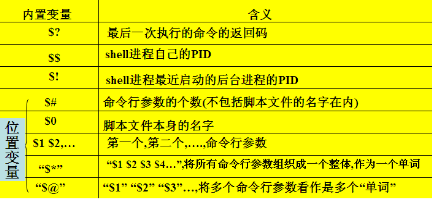
\includegraphics[width=9cm]{c8.shell.buildin.01.png}\\
    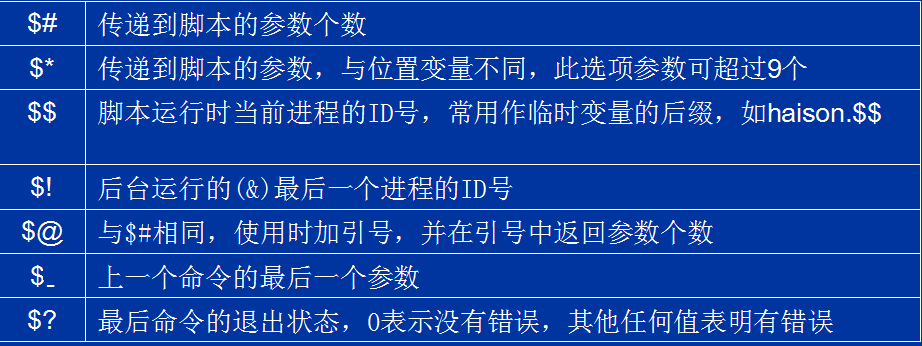
\includegraphics[width=9cm]{c8.shell.buildin.02.png}
  \end{figure}
\end{frame}

\begin{frame}[fragile]
  \frametitle{编程起步 | 特殊变量 | 脚本参数}
  Users often need to pass parameter values to a script, such as a filename, date, etc. Scripts will take different paths or arrive at different values according to the parameters (command arguments) that are passed to them. These values can be text or numbers. Within a script, the parameter or an argument is represented with a \verb|$| and a number.
  \begin{figure}
    \centering
    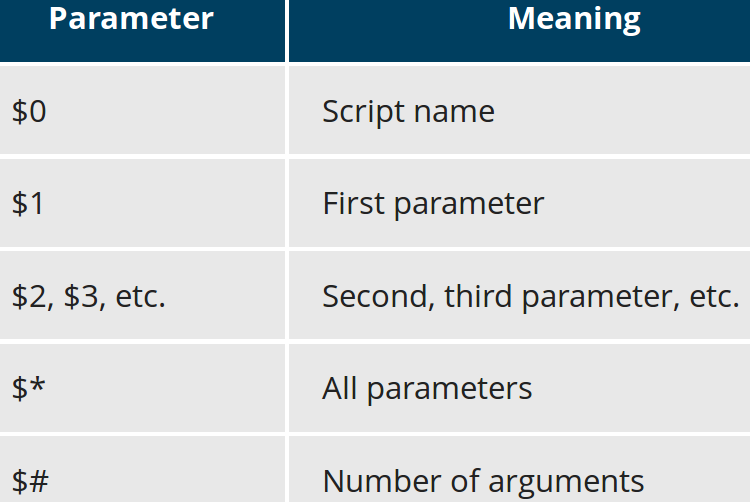
\includegraphics[width=9cm,height=5cm]{c8.script.parameter.png}
  \end{figure}
\end{frame}

\begin{frame}[fragile]
  \frametitle{编程起步 | 特殊变量 | \alert{脚本参数}}
\begin{lstlisting}
#!/bin/bash
echo The name of this program is: $0
echo The first argument passed from the command line is: $1
echo The second argument passed from the command line is: $2
echo The third argument passed from the command line is: $3
echo All of the arguments passed from the command line are : $*
echo
echo All done with $0
\end{lstlisting}
\end{frame}

\begin{frame}
  \frametitle{编程起步 | 特殊变量 | 脚本参数}
  \begin{figure}
    \centering
    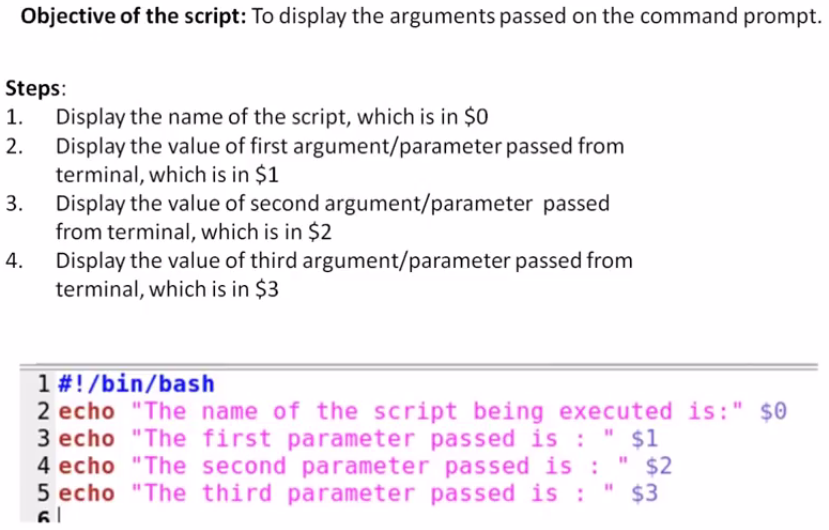
\includegraphics[width=11cm]{c8.script.parameter.example.png}
  \end{figure}
\end{frame}

\begin{frame}
  \frametitle{编程起步 | 特殊变量 | \alert{演示}}
  \begin{figure}
    \centering
    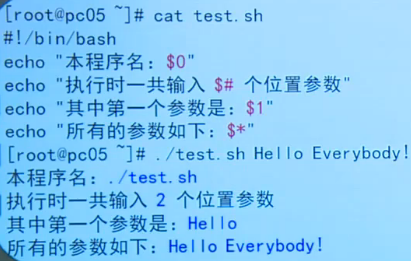
\includegraphics[width=10cm]{c8.shell.buildin.05.png}
  \end{figure}
\end{frame}

\subsection{退出状态}
\begin{frame}[fragile]
  \frametitle{编程起步 | \alert{退出状态}}
  \begin{block}{退出状态}
    \begin{itemize}
      \item 退出状态(exit status)是每个命令在完成时返回的一个数值。
      \item 通常情况下,如果命令执行成功,返回退出状态0;如果不成功,则返回1(非零的数值)。
      \item 有些命令由于特殊原因会返回额外的退出状态。
      \item \verb|exit 0|
    \end{itemize}
  \end{block}
  \vspace{-0.3cm}
  \begin{figure}
    \centering
    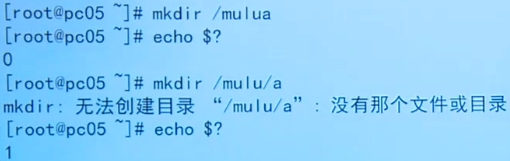
\includegraphics[width=9cm,height=2.1cm]{c8.shell.exit.01.png}\\
    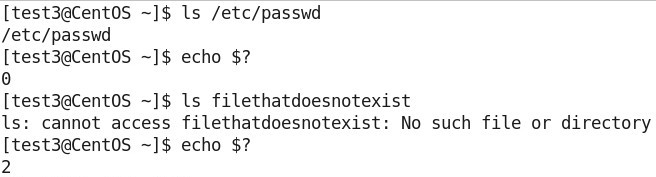
\includegraphics[width=9cm,height=2.1cm]{c8.shell.exit.10.jpg}
  \end{figure}
\end{frame}

\section{流程控制}
\begin{frame}
  \frametitle{流程控制 | 简介}
  \begin{block}{流程控制}
    流程控制(flow control)允许程序做出判断:程序计算条件的值,并根据这些条件执行相应的操作。
  \end{block}
  \pause
  \begin{block}{\alert{分类}}
    \begin{enumerate}
      \item 条件流程控制(conditional flow control):根据特定的约束是否满足来决定是否执行某个代码段
      \item 迭代流程控制(iterative flow control):代码块重复或迭代,直到满足某个条件为止
    \end{enumerate}
  \end{block}
\end{frame}

\begin{frame}
  \frametitle{流程控制 | 条件 vs. 迭代}
  \begin{figure}
    \centering
    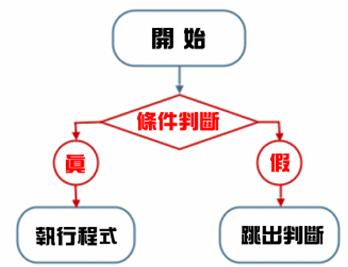
\includegraphics[width=6cm]{c8.conditional.01.jpg}
    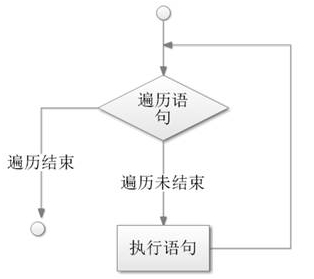
\includegraphics[width=6cm]{c8.iterative.jpg}
  \end{figure}
\end{frame}

\subsection{条件流程控制}
\begin{frame}
  \frametitle{流程控制 | 条件流程控制 | if-then | Introduction}
  Conditional decision making using an \textbf{if} statement, is a basic
  construct that any useful programming or scripting language must
  have.\\
  \vspace{0.3cm}
  When an \textbf{if} statement is used, the ensuing actions depend on the evaluation of specified conditions such as:
  \begin{itemize}
    \item Numerical or string comparisons
    \item Return value of a command (0 for success)
    \item File existence or permissions
  \end{itemize}
\end{frame}

\begin{frame}[fragile]
  \frametitle{流程控制 | 条件流程控制 | if-then | Syntax}
\begin{lstlisting}
# compact form
if TEST-COMMANDS; then CONSEQUENT-COMMANDS; fi

# more general definition
if condition
then
  statements
else
  statements
fi

if [ -f /etc/passwd  ] ; then
  ACTION
fi
\end{lstlisting}
\end{frame}

\begin{frame}
  \frametitle{流程控制 | 条件流程控制 | if-then | Example}
  \begin{figure}
    \centering
    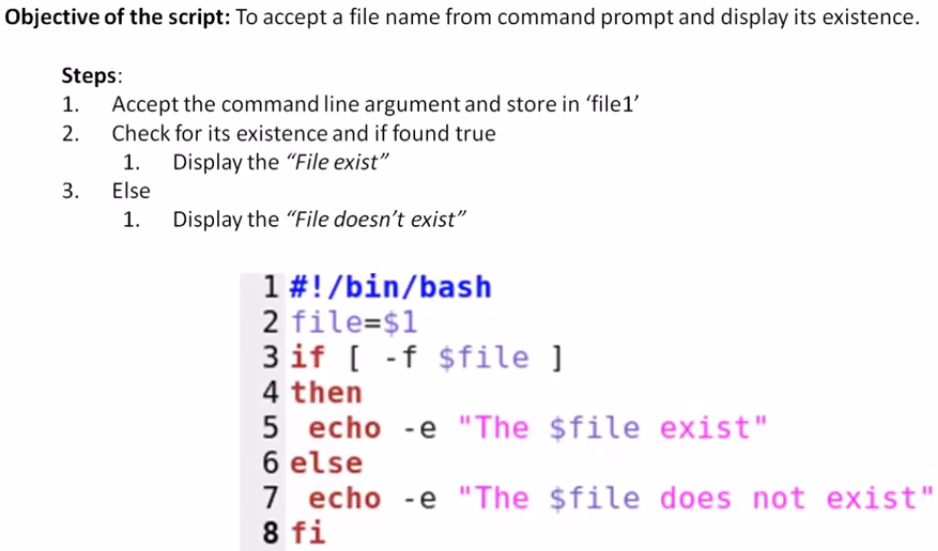
\includegraphics[width=11cm]{c8.if.example.10.png}
  \end{figure}
\end{frame}

\begin{frame}
  \frametitle{流程控制 | 条件流程控制 | if-then | Example}
  \begin{figure}
    \centering
    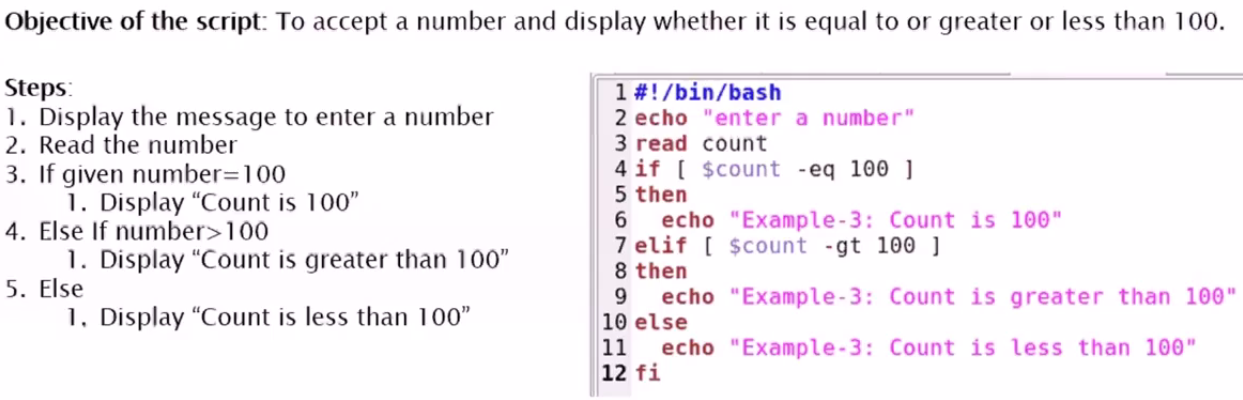
\includegraphics[width=12cm]{c8.if.example.11.png}
  \end{figure}
\end{frame}

\begin{frame}
  \frametitle{流程控制 | 条件流程控制 | if-then | Example}
  \begin{figure}
    \centering
    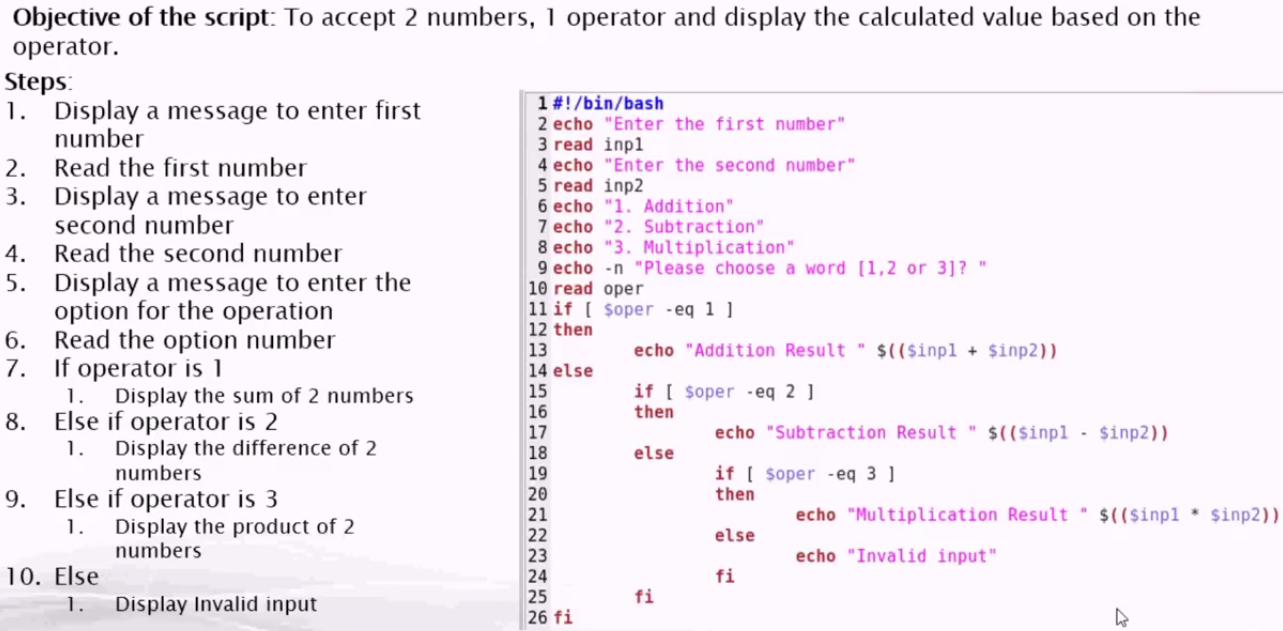
\includegraphics[width=12cm]{c8.if.example.12.png}
  \end{figure}
\end{frame}

\begin{frame}
  \frametitle{流程控制 | 条件流程控制 | if-then | Example}
  \begin{figure}
    \centering
    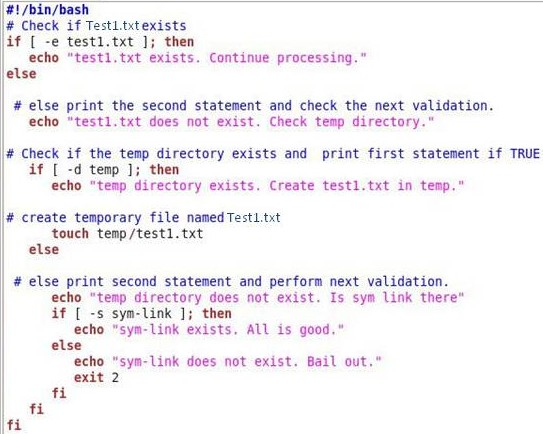
\includegraphics[width=9.5cm]{c8.if.example.13.jpg}
  \end{figure}
\end{frame}

\begin{frame}
  \frametitle{流程控制 | 条件流程控制 | if-then | 逻辑流程}
  \begin{figure}
    \centering
    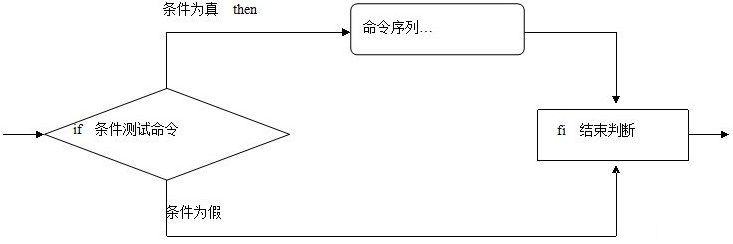
\includegraphics[width=11cm]{c8.if.01.jpg}
  \end{figure}
\end{frame}

\begin{frame}[fragile]
  \frametitle{流程控制 | 条件流程控制 | if-then | \alert{语法}}
\begin{lstlisting}
if some_condition
then
  something happens
fi
\end{lstlisting}
\end{frame}

\begin{frame}[fragile]
  \frametitle{流程控制 | 条件流程控制 | if-then | 实例}
\begin{lstlisting}
#!/bin/bash
echo "Guess the secret color"
read COLOR
if [ $COLOR = "purple" ]
then
  echo "You are correct."
fi
\end{lstlisting}
\pause
\begin{lstlisting}
#!/bin/bash
if [ ${SHELL} = "/bin/bash" ]; then
  echo "your login shell is the bash"
else
  echo "your login shell is ${SHELL}"
fi
\end{lstlisting}
\end{frame}

\begin{frame}
  \frametitle{流程控制 | 条件流程控制 | if-then | 逻辑流程}
  \begin{figure}
    \centering
    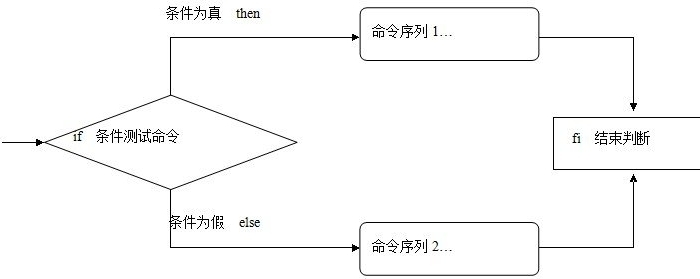
\includegraphics[width=11cm]{c8.if.02.jpg}
  \end{figure}
\end{frame}

\begin{frame}[fragile]
  \frametitle{流程控制 | 条件流程控制 | if-then | \alert{语法}}
\begin{lstlisting}
if some_condition
then
  something happens
else
  something happens
fi
\end{lstlisting}
\end{frame}

\begin{frame}[fragile]
  \frametitle{流程控制 | 条件流程控制 | if-then | 实例}
\begin{lstlisting}
#!/bin/bash

echo "Guess the secret color"

read COLOR
if [ $COLOR = "purple" ]
then
  echo "You are correct."
else
  echo "Your guess was incorrect."
fi
\end{lstlisting}
\end{frame}

\begin{frame}
  \frametitle{流程控制 | 条件流程控制 | if-then | 逻辑流程}
  \begin{figure}
    \centering
    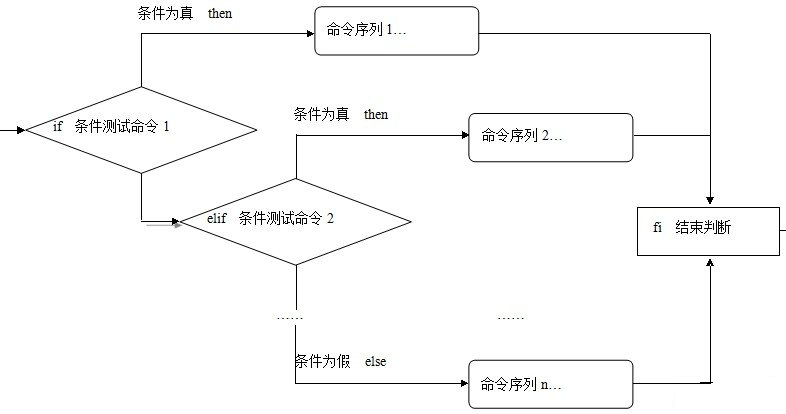
\includegraphics[width=11cm]{c8.if.03.jpg}
  \end{figure}
\end{frame}

\begin{frame}[fragile]
  \frametitle{流程控制 | 条件流程控制 | if-then | \alert{语法}}
\begin{lstlisting}
if some_condition
then
  something happens
elif other_condition
then
  something happens
else
  something happens
fi
\end{lstlisting}
\end{frame}

\begin{frame}[fragile]
  \frametitle{流程控制 | 条件流程控制 | if-then | 实例}
\begin{lstlisting}
#!/bin/bash

echo "Guess the secret color"

read COLOR
if [ $COLOR = "purple" ]
then
  echo "You are correct."
elif [ $COLOR = "blue" ]
then
  echo "You are close."
else
  echo "Your guess was incorrect."
fi
\end{lstlisting}
\end{frame}

\begin{frame}
  \frametitle{流程控制 | 条件流程控制 | if-then | \alert{实例}}
  \begin{figure}
    %\centering
    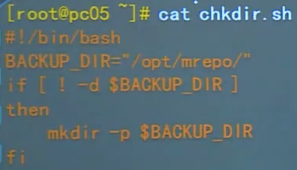
\includegraphics[width=5.7cm]{c8.if.example.01.png}\quad
    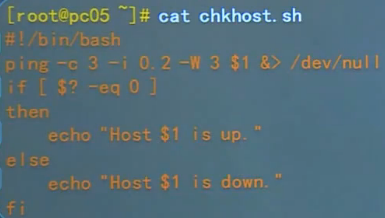
\includegraphics[width=5.8cm]{c8.if.example.02.png}\\
    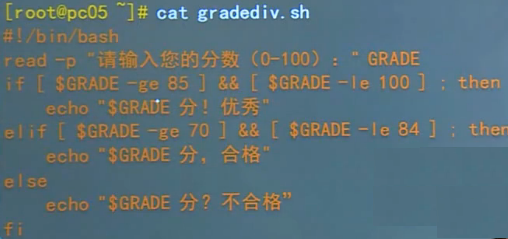
\includegraphics[width=9cm]{c8.if.example.03.png}
  \end{figure}
\end{frame}

\begin{frame}
  \frametitle{流程控制 | 条件流程控制 | if-then | 补充说明}
  \begin{figure}
    \centering
    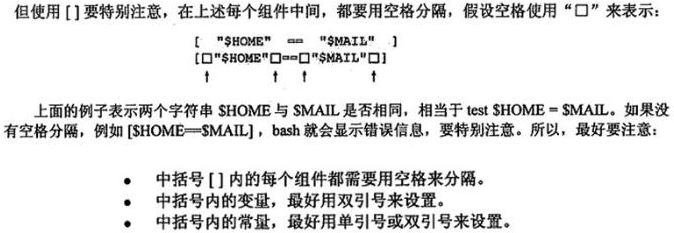
\includegraphics[width=12cm]{c8.if.04.jpg}\\
    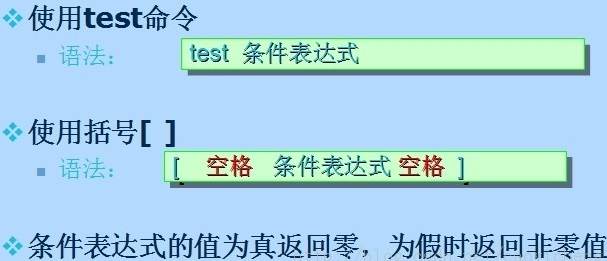
\includegraphics[width=10cm,height=3.5cm]{c8.test.01.jpg}
  \end{figure}
\end{frame}

\begin{frame}[fragile]
  \frametitle{流程控制 | 条件流程控制 | \alert{test}}
  \begin{block}{test}
    \begin{itemize}
      \item test命令用于计算条件的值。
      \item 方括号在语法上与test命令等价。
      \item 方括号中的空格很重要,要确保方括号前后的空格。
    \end{itemize}
  \end{block}
  \pause
\begin{lstlisting}
if [ $COLOR = "purple" ]
if (test $COLOR = "purple")

# 测试文件是否存在
if [ -e filename ]
if (test -e filename)
\end{lstlisting}
\end{frame}

\begin{frame}[fragile]
  \frametitle{流程控制 | 条件流程控制 | test | \alert{文件测试}}
  \begin{table}
    \centering
    \rowcolors[]{1}{blue!20}{blue!10}
    \begin{tabularx}{\textwidth}{ccX}
      \hline
      \rowcolor{blue!50}测试 & 助记 & 功能\\
      \hline
      -d & Directory & 文件存在并且是目录\\
      -e & Exist & 指定的文件存在\\
      -f & File & 文在存在并且是普通文件\\
      -G & Group & 执行命令的用户属于文件所属组的成员\\
      -nt & Newer Than & file1 -nt file2,前一个文件比后一个文件新\\
      -ot & Older Than & file1 -ot file2,前一个文件比后一个文件老\\
      -O & Owner & 执行命令的用户是文件的所有者\\
      -r & Read & 执行命令的用户拥有对文件的读取权限\\
      -s & Size & 文在存在并且不为空\\
      -w & Write & 执行命令的用户拥有对文件的写入权限\\
      -x & eXecute & 执行命令的用户拥有对文件的执行权限\\
      \hline
    \end{tabularx}
  \end{table}
  You can view the full list of file conditions using the command \verb|man 1 test|.
\end{frame}

\begin{frame}
  \frametitle{流程控制 | 条件流程控制 | test | 文件测试}
  \begin{figure}
    \centering
    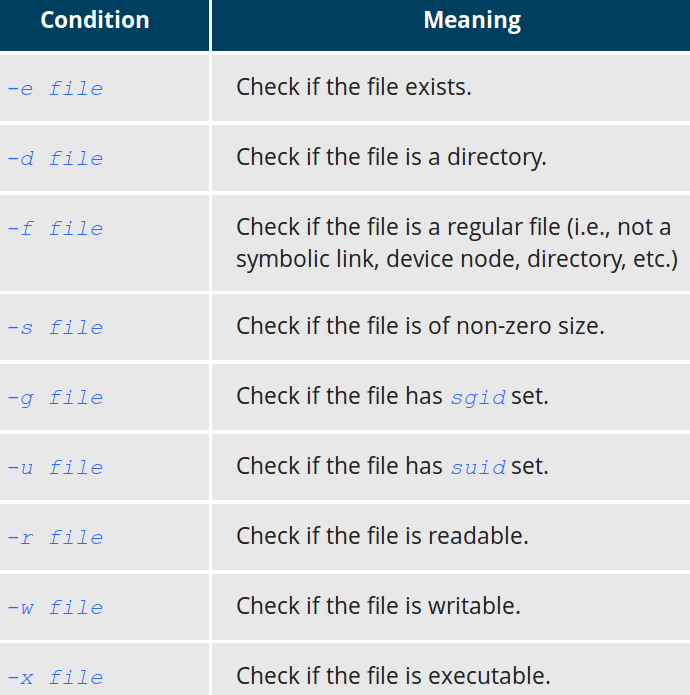
\includegraphics[width=11cm,height=7cm]{c8.test.file.10.png}
  \end{figure}
\end{frame}

\begin{frame}
  \frametitle{流程控制 | 条件流程控制 | test | 文件测试}
  \begin{figure}
    \centering
    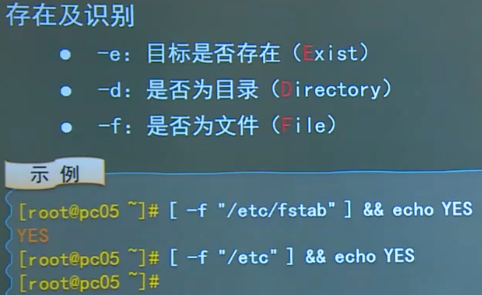
\includegraphics[width=8cm,height=3.8cm]{c8.test.file.01.png}\\
    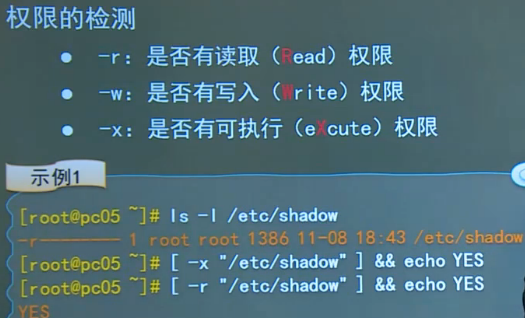
\includegraphics[width=8cm,height=3.8cm]{c8.test.file.02.png}
  \end{figure}
\end{frame}

\begin{frame}
  \frametitle{流程控制 | 条件流程控制 | 比较运算符 | \alert{字符串比较}}
  \begin{table}
    \centering
    \rowcolors[]{1}{blue!20}{blue!10}
    \begin{tabularx}{\textwidth}{ccX}
      \hline
      \rowcolor{blue!50}运算符 & 示例 & 功能\\
      \hline
      = & stringA=stringB & stringA与stringB相同,与==等价\\
      != & stringA!=stringB & stringA与stringB不同\\
      > & stringA>stringB & stringA大于stringB\\
      < & stringA<stringB & stringA小于stringB\\
      -z & -z string & string为空\\
      -n & -n string & string非空\\
      \hline
    \end{tabularx}
  \end{table}
  \begin{figure}
    \centering
    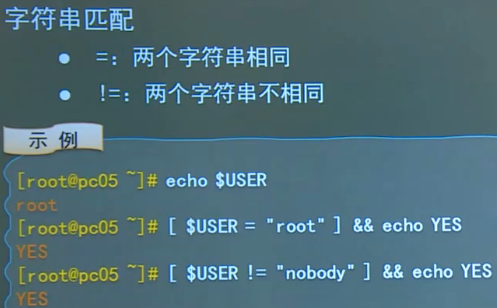
\includegraphics[width=9cm,height=4cm]{c8.test.string.01.png}
  \end{figure}
\end{frame}

\begin{frame}
  \frametitle{流程控制 | 条件流程控制 | 比较运算符 | 字符串比较}
  \begin{figure}
    \centering
    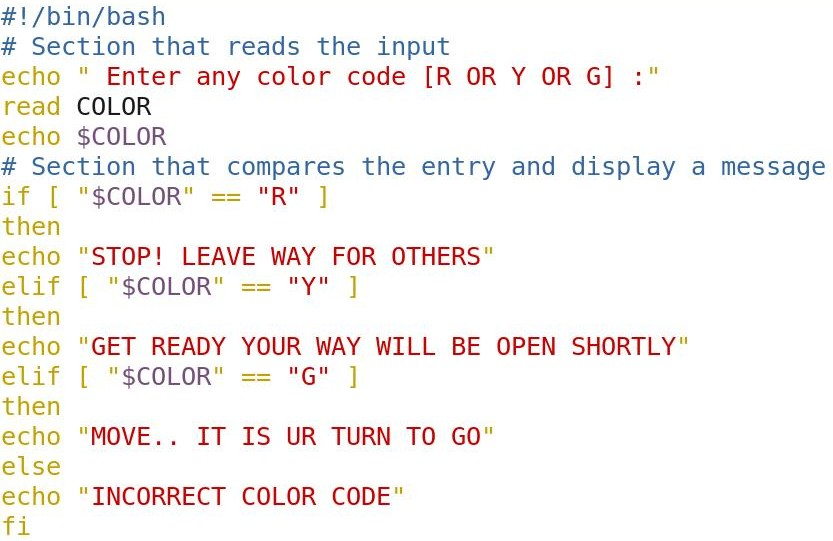
\includegraphics[width=11cm]{c8.test.string.10.jpg}
  \end{figure}
\end{frame}

\begin{frame}[fragile]
  \frametitle{流程控制 | 条件流程控制 | 比较运算符 | 字符串操作}
  A \textbf{string variable} contains a sequence of text characters. It can include letters, numbers, symbols and punctuation marks. Some examples: \verb|abcde|, \verb|123|, \verb|abcde 123|, \verb|abcde-123|, \verb|&acbde=%123|.\\
  \vspace{0.2cm}
  String \textbf{operators} include those that do comparison, sorting, and finding the length.
  \begin{figure}
    \centering
    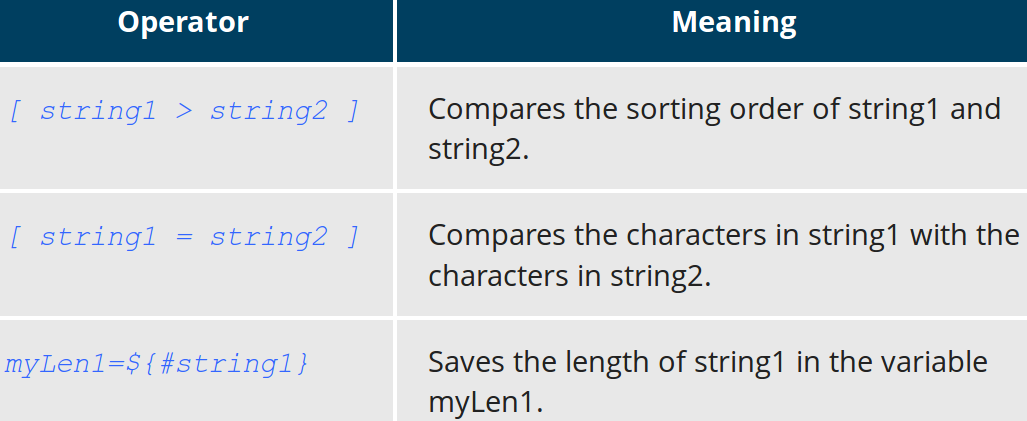
\includegraphics[width=11cm]{c8.string.01.png}
  \end{figure}
\end{frame}

%\begin{frame}
  %\frametitle{流程控制 | 条件流程控制 | 比较运算符 | 字符串操作}
  %\begin{figure}
    %\centering
    %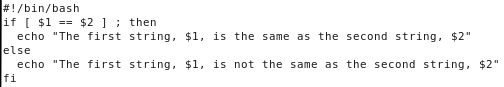
\includegraphics[width=12cm]{c8.string.02.png}\\
    %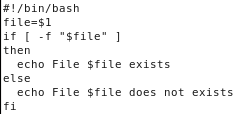
\includegraphics[width=7cm]{c8.string.03.png}
  %\end{figure}
%\end{frame}

\begin{frame}[fragile]
  \frametitle{流程控制 | 条件流程控制 | 比较运算符 | 字符串操作}
  At times, you may not need to compare or use an entire string.\\
  \vspace{0.2cm}
  To extract the first character of a string we can specify: \verb|${string:0:1}|. Here 0 is the offset in the string (i.e., which character to begin from) where the extraction needs to start and 1 is the number of characters to be extracted.\\
  \vspace{0.2cm}
  To extract all characters in a string after a dot (.), use the following expression: \verb|${string#*.}|.
  \begin{figure}
    \centering
    
\includegraphics[width=11cm]{c8.string.04.jpg}
  \end{figure}
\end{frame}

\begin{frame}
  \frametitle{流程控制 | 条件流程控制 | 比较运算符 | 字符串操作}
  \begin{figure}
    \centering
    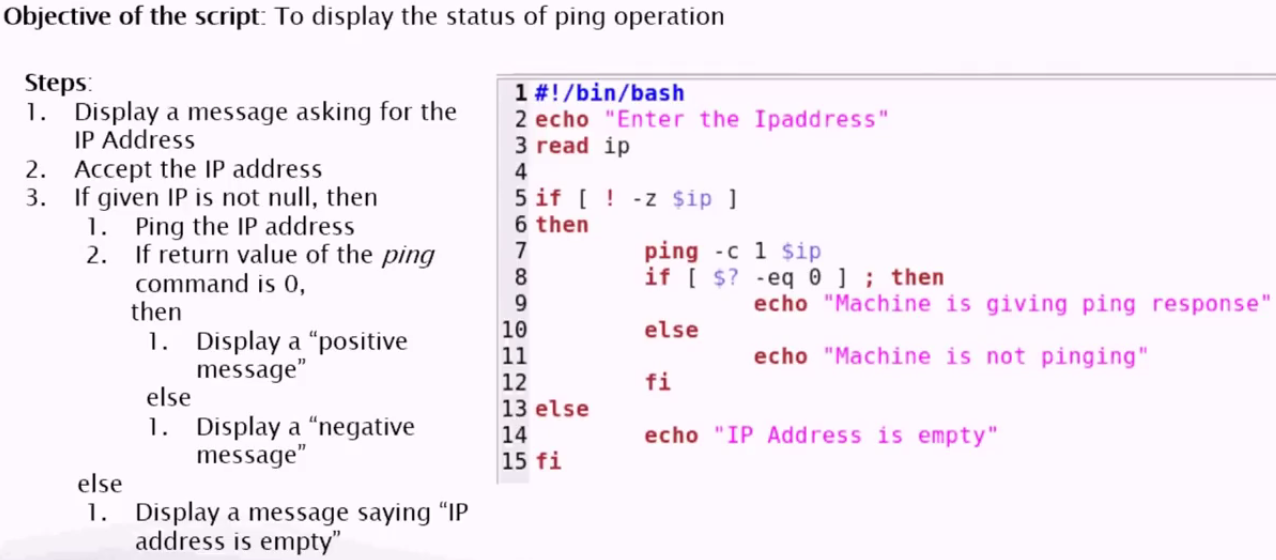
\includegraphics[width=12cm]{c8.string.05.png}
  \end{figure}
\end{frame}

\begin{frame}
  \frametitle{流程控制 | 条件流程控制 | 比较运算符 | 字符串操作}
  \begin{figure}
    \centering
    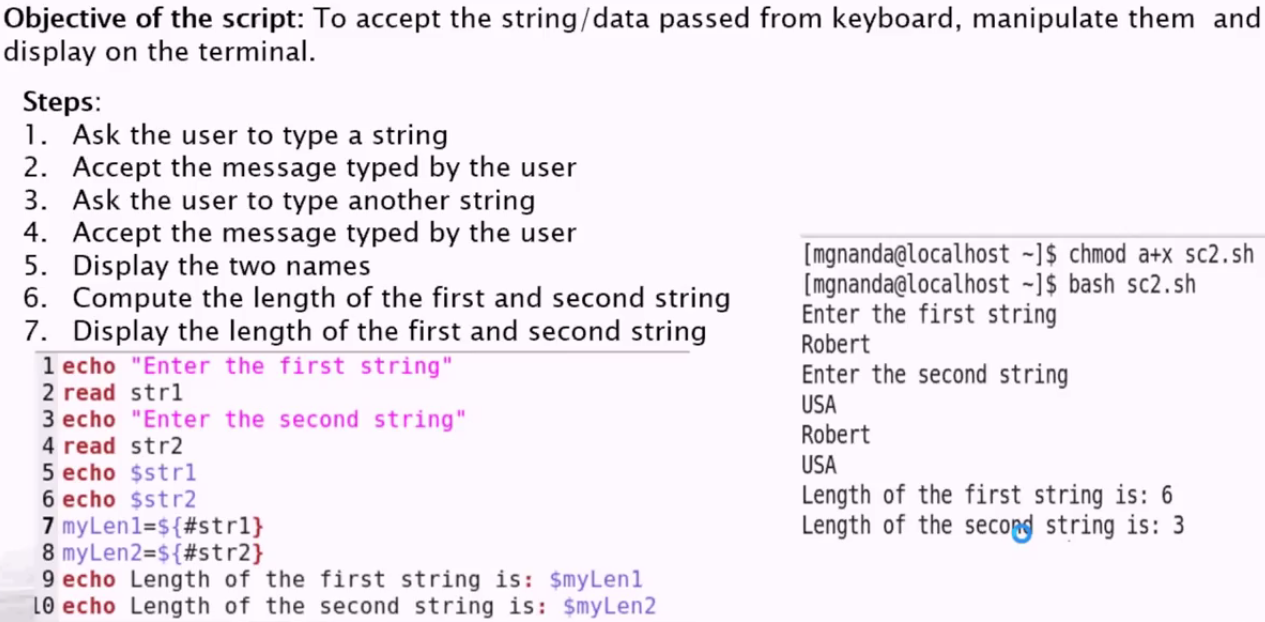
\includegraphics[width=12cm]{c8.string.06.png}
  \end{figure}
\end{frame}

\begin{frame}
  \frametitle{流程控制 | 条件流程控制 | 比较运算符 | \alert{整数值比较}}
  \begin{table}
    \centering
    \rowcolors[]{1}{blue!20}{blue!10}
    \begin{tabularx}{0.7\textwidth}{ccX}
      \hline
      \rowcolor{blue!50}运算符 & 助记 & 功能\\
      \hline
      -eq & EQual & 等于\\
      -ne & Not Equal & 不等于\\
      -gt & Greater Than & 大于\\
      -lt & Lesser Than & 小于\\
      -ge & Greater or Equal & 大于等于\\
      -le & Lesser or Equal & 小于等于\\
      \hline
    \end{tabularx}
  \end{table}
  \begin{figure}
    \centering
    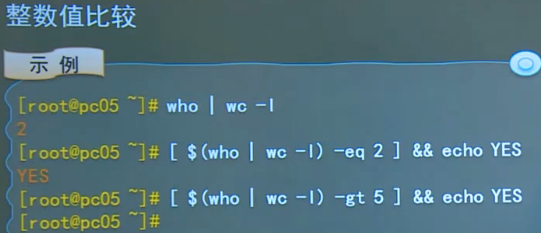
\includegraphics[width=9cm,height=4cm]{c8.test.number.04.png}
  \end{figure}
\end{frame}

\begin{frame}
  \frametitle{流程控制 | 条件流程控制 | 比较运算符 | 整数值比较}
  \begin{figure}
    \centering
    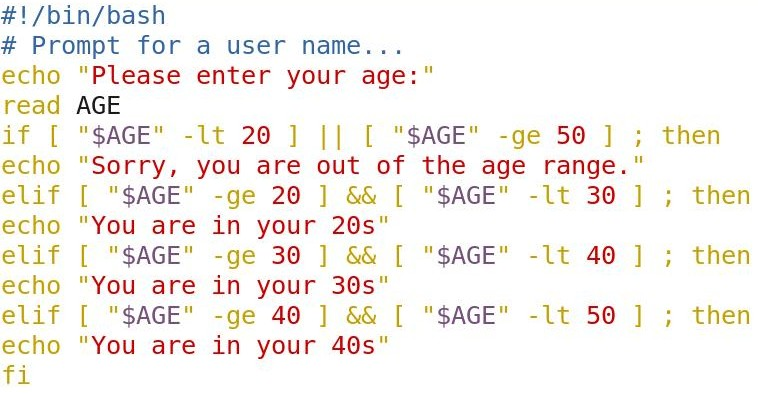
\includegraphics[width=11cm]{c8.test.number.11.jpg}
  \end{figure}
\end{frame}

\begin{frame}
  \frametitle{流程控制 | 条件流程控制 | 比较运算符 | 整数值比较}
  \begin{figure}
    \centering
    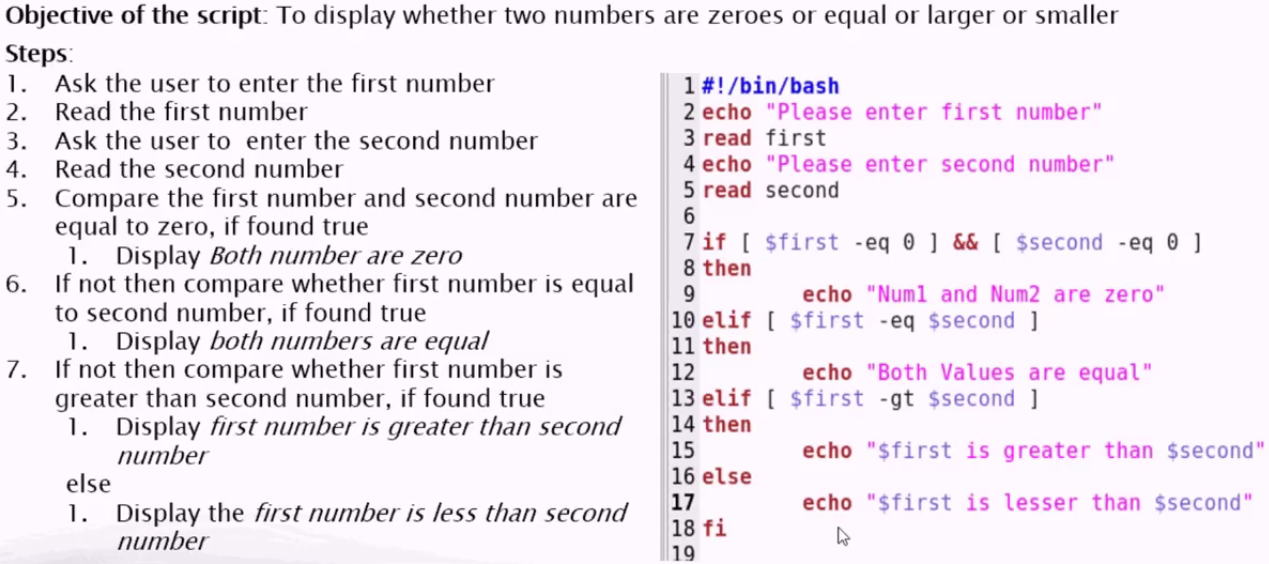
\includegraphics[width=12cm]{c8.test.number.12.png}
  \end{figure}
\end{frame}

\begin{frame}[fragile]
  \frametitle{流程控制 | 条件流程控制 | 比较运算符 | \alert{算数运算}}
  \begin{description}
    \item[\$(( ))] shell内置的算数运算格式
    \item[\${[} {]}] 将中括号内的表达式作为数学运算先计算结果再输出
    \item[let] 表示数学运算
    \item[expr] 用于整数值运算,每一项用空格隔开
  \end{description}
\end{frame}

\begin{frame}[fragile]
  \frametitle{流程控制 | 条件流程控制 | 比较运算符 | 算术运算}
  Arithmetic expressions can be evaluated in the following three ways (spaces are important!):
  \begin{itemize}
    \item Using the \textbf{expr} utility: \textbf{expr} is a standard but somewhat deprecated program. The syntax is as follows: \verb|expr 8 + 8|; \verb|echo $(expr 8 + 8)|
    \item Using the \verb|$((...))| syntax: This is the built-in shell format. The syntax is as follows: \verb|echo $((x+1))|
    \item Using the built-in shell command \verb|let|.  The syntax is as follows: \verb|let x=( 1 + 2 ); echo $x|
  \end{itemize}
  In modern shell scripts the use of \textbf{expr} is better replaced with \verb|var=$((...))|.
\end{frame}

\begin{frame}[fragile]
  \frametitle{流程控制 | 条件流程控制 | 比较运算符 | 算数运算}
\begin{lstlisting}
# 默认将变量作为文本字符串
MYVAR=1
MYVAR=$MYVAR+1
echo $MYVAR # 输出:1+1

# 需要用特定的方法进行算数运算
MYVAR=`expr $MYVAR + 1`
echo $MYVAR # 输出:2
\end{lstlisting}
\end{frame}

\begin{frame}[fragile]
  \frametitle{流程控制 | 条件流程 | 比较运算符 | 算数运算 | \alert{四种方法}}
\begin{lstlisting}
var=1 # var:1

# 第一种方法:$(( ))
var=$(($var+1)) # var:2
((var++)) # var:3

# 第二种方法:$[ ]
var=$[$var+1] # var:4

# 第三种方法:let
let var+=1 # var:5

# 第四种方法:expr(注意加号两边的空格,否则还是按照字符串的方式赋值)
var=$(expr $var + 1) # var:6,不建议使用
var=`expr $var + 1` # var:7,强烈不建议使用
\end{lstlisting}
\end{frame}

\begin{frame}[fragile]
  \frametitle{流程控制 | 条件流程控制 | 比较运算符 | 算数运算}
  \begin{figure}
    \centering
    \includegraphics[width=5cm]{c8.expr.02.png}
    \includegraphics[width=7cm]{c8.expr.01.png}
    \vspace{0.3cm}
    \includegraphics[width=12cm]{c8.expr.03.png}
  \end{figure}
\end{frame}

\begin{frame}
  \frametitle{流程控制 | 条件流程控制 | \alert{多个条件}}
  \begin{figure}
    \centering
    \includegraphics[width=12cm]{c8.andor.01.jpg}
  \end{figure}
\end{frame}

\begin{frame}[fragile]
  \frametitle{流程控制 | 条件流程控制 | 多个条件}
\begin{lstlisting}
# 逻辑运算符and(&&,-a)
if [ condition1 -a condition2 ]
# if [ condition1 ] && [ condition2 ]
then
  some action
fi

# 等价于
if [ condition1 ]
then
  if [ condition2 ]
  then
    some action
  fi
fi
\end{lstlisting}
\end{frame}

\begin{frame}[fragile]
  \frametitle{流程控制 | 条件流程控制 | 多个条件}
\begin{lstlisting}
# 逻辑运算符or(||,-o)
if [ condition1 -o condition2 ]
# if [ condition1 ] || [ condition2 ]
then
  some action
fi

# 等价于
if [ condition1 ]
then
  some action
elif [ condition2 ]
then
  the same action
fi
\end{lstlisting}
\end{frame}

\begin{frame}[fragile]
  \frametitle{流程控制 | 条件流程控制 | 多个条件}
  \textbf{Boolean} expressions evaluate to either \textbf{TRUE} or \textbf{FALSE}, and results are obtained using the various Boolean operators.
  \begin{figure}
    \centering
    \includegraphics[width=11cm]{c8.boolean.png}
  \end{figure}
\end{frame}

\begin{frame}[fragile]
  \frametitle{流程控制 | 条件流程控制 | 多个条件}
  Note that if you have multiple conditions strung together with the \verb|&&| operator processing stops as soon as a condition evaluates to false.  For example if you have \verb|A && B && C| and A is true but B is false, C will never be executed.\\
  \vspace{0.3cm}
  Likewise if you are using the \verb=||= operator, processing stops as soon as anything is true. For example if you have \verb=A || B || C= and A is false and B is true, you will also never execute C.
\end{frame}

\begin{frame}[fragile]
  \frametitle{流程控制 | 条件流程控制 | 补充}
  \begin{itemize}
    \item 在[\ ]表达式中,不直接支持>、<运算符,需要加转义字符,表示字符串大小比较,以ASCII码位置作为比较。
    \item 在[\ ]表达式中,逻辑运算符||、\&\&需要分别用-o和-a表示。
    \item {[[}\ {]]}运算符只是[\ ]运算符的扩充。能够支持>、>符号运算,不再需要转义符,它还是以字符串比较大小。
    \item {[[}\ {]]}运算符里面支持逻辑运算符||和\&\&。
  \end{itemize}
  In modern scripts you may see doubled brackets as in \verb|[[ -f /etc/passwd ]]|. This is not an error. It is never wrong to do so and it avoids some subtle problems such as referring to an empty environment variable without surrounding it in double quotes.
\end{frame}

\begin{frame}
  \frametitle{流程控制 | 条件流程控制 | 运算符 | 汇总(1/3)}
  \begin{figure}
    \centering
    \includegraphics[width=11cm]{c8.operator.01.png}
  \end{figure}
\end{frame}

\begin{frame}
  \frametitle{流程控制 | 条件流程控制 | 运算符 | 汇总(2/3)}
  \begin{figure}
    \centering
    \includegraphics[width=10cm]{c8.operator.02.png}
  \end{figure}
\end{frame}

\begin{frame}
  \frametitle{流程控制 | 条件流程控制 | 运算符 | 汇总(3/3)}
  \begin{figure}
    \centering
    \includegraphics[width=10cm]{c8.operator.03.png}
  \end{figure}
\end{frame}

\subsection{选择流程控制}
\begin{frame}[fragile]
  \frametitle{流程控制 | 选择流程控制 | select | \alert{语法}}
  \begin{block}{作用}
    select表达式是bash的一种扩展应用,擅长于交互式场合。它把关键字中的每一项做成表单,用户可以从中进行选择。
    \begin{enumerate}
      \item 自动用1、2、3、4列出菜单(没有echo指令,自动显示菜单)
      \item 自动read输入选择(没有read指令,自动输入)
      \item 赋值给变量(没有赋值指令,自动输入数字后,赋值字符串给变量)
    \end{enumerate}
  \end{block}
  \pause
  \begin{block}{语法}
\begin{lstlisting}
select var in WORDS
do
  command(s)
done
... now $var can be used ...
\end{lstlisting}
  \end{block}
\end{frame}

\begin{frame}[fragile]
  \frametitle{流程控制 | 选择流程控制 | select | \alert{实例}}
\begin{lstlisting}
#!/bin/bash
echo "What is your favourite OS?"
select var in "Linux" "Free BSD" "Other"
do
  break
done
echo "You have selected $var"

# 运行结果
What is your favourite OS?
1) Linux
2) Free BSD
3) Other
#? 1
You have selected Linux
\end{lstlisting}
\end{frame}

\begin{frame}
  \frametitle{流程控制 | 选择流程控制 | select | 补充}
  \begin{itemize}
    \item select本身就是一个循环,break是当选择后就跳出循环
    \item select输入选择是数字,但变量值却是字符串
    \item 一般与case语句配合使用
  \end{itemize}
\end{frame}

\begin{frame}[fragile]
  \frametitle{流程控制 | 选择流程控制 | case | Introduction}
  The \verb|case| statement is used in scenarios where the actual value of a variable can lead to different execution paths. \verb|case| statements are often used to handle command-line options.
  \begin{figure}
    \centering
    \includegraphics[width=11cm]{c8.case.10.jpg}
  \end{figure}
\end{frame}

\begin{frame}
  \frametitle{流程控制 | 选择流程控制 | case | Strcture}
  \begin{figure}
    \centering
    \includegraphics[width=6cm]{c8.case.11.jpg}
  \end{figure}
\end{frame}

\begin{frame}[fragile]
  \frametitle{流程控制 | 选择流程控制 | case | Syntax}
\begin{lstlisting}
case expression in
  pattern1) execute commands;;
  pattern2) execute commands;;
  pattern3) execute commands;;
  pattern4) execute commands;;
  * )       execute some default commands or nothing ;;
esac
\end{lstlisting}
\end{frame}

\begin{frame}
  \frametitle{流程控制 | 选择流程控制 | case | Example}
  \begin{figure}
    \centering
    \includegraphics[width=11cm]{c8.case.12.png}
  \end{figure}
\end{frame}

\begin{frame}
  \frametitle{流程控制 | 选择流程控制 | case | 逻辑流程}
  \begin{figure}
    \centering
    \includegraphics[width=12cm]{c8.case.01.png}
  \end{figure}
\end{frame}

\begin{frame}[fragile]
  \frametitle{流程控制 | 选择流程控制 | case | \alert{语法}}
  \begin{block}{作用}
    case表达式可以用来匹配一个给定的字符串,而不是数字。
  \end{block}
  \pause
\begin{lstlisting}
case expression in
  pattern1)
    action1
    ;;
  pattern2)
    action2
    ;;
  *)
    default action
    ;;
esac
\end{lstlisting}
\end{frame}

\begin{frame}[fragile]
  \frametitle{流程控制 | 选择流程控制 | case | 说明}
  \begin{block}{pattern}
    pattern是正则表达式,可以用下面的字符:
    \begin{description}
      \item[*] 任意字符串
      \item[?] 任意单个字符
      \item[{[}abc{]}] a、b或c单个字符其中之一
      \item[{[}a-n{]}] 从a到n的任意一个字符
      \item[|] 多重选择
    \end{description}
  \end{block}
\end{frame}

\begin{frame}[fragile]
  \frametitle{流程控制 | 选择流程控制 | case | 实例}
\begin{lstlisting}
#!/bin/bash
case "$1" in
  start)
    sleep 3600 &
    ;;
  stop)
    pkill -x "sleep"
    ;;
  *)
    echo "用法:$0 {start|stop}"
    ;;
esac
\end{lstlisting}
\end{frame}

\begin{frame}[fragile]
  \frametitle{流程控制 | 选择流程控制 | case | \alert{实例}}
\begin{lstlisting}
#!/bin/bash
read -p "请输入一个字符,并按Enter键确认:" KEY
case "$KEY" in
  [a-z]|[A-Z])
    echo "您输入的是——字母。"
    ;;
  [0-9])
    echo "您输入的是——数字。"
    ;;
  *)
    echo "您输入的是——空格、功能键或其他控制字符。"
    ;;
esac
\end{lstlisting}
\end{frame}

\begin{frame}[fragile]
  \frametitle{流程控制 | 选择流程控制 | case | \alert{实例}}
\begin{lstlisting}
# smartzip,自动解压bzip2、gzip和zip类型的压缩文件
#!/bin/bash

ftype="$(file "$1")"
case "$ftype" in
  "$1: Zip archive"*)
    unzip "$1" ;;
  "$1: gzip compressed"*)
    gunzip "$1" ;;
  "$1: bzip2 compressed"*)
    bunzip2 "$1" ;;
  *)
    echo "File $1 can not be uncompressed with smartzip";;
esac
\end{lstlisting}
\end{frame}

\begin{frame}[fragile]
  \frametitle{流程控制 | 选择流程控制 | \alert{select \& case}}
\begin{lstlisting}[basicstyle=\footnotesize\tt]
#!/bin/bash

select DRINK in tea cofee water juice appe all none
do
  case $DRINK in
    tea|cofee|water|all) 
      echo "Go to canteen"
      ;;
    juice|appe)
      echo "Available at home"
      ;;
    none) 
      break 
      ;;
    *)
      echo "ERROR: Invalid selection" 
      ;;
  esac
done
\end{lstlisting}
\end{frame}

\subsection{迭代流程控制}
\begin{frame}[fragile]
  \frametitle{流程控制 | 迭代流程控制 | Introduction}
  By using \textbf{looping constructs}, you can execute one or more
  lines of code repetitively. Usually you do this until a conditional
  test returns either true or false as is required.\\
  \vspace{0.3cm}
  Three type of loops are often used in most programming languages:
  \begin{itemize}
    \item \verb|for|
    \item \verb|while|
    \item \verb|until|
  \end{itemize}
  All these loops are easily used for repeating a set of statements until the exit condition is true.
\end{frame}

\begin{frame}[fragile]
  \frametitle{流程控制 | 迭代流程控制 | while | Introduction}
  The \verb|while| loop repeats a set of statements as long as the control command returns true.\\
  \vspace{-0.2cm}
\begin{lstlisting}
while condition is true
do
  Commands for execution
done
\end{lstlisting}
  \vspace{-0.1cm}
  The set of commands that need to be repeated should be enclosed between \verb|do| and \verb|done|. You can use any command or operator as the condition.  Often it is enclosed within square brackets (\verb|[]|).\\
  \vspace{-0.2cm}
  \begin{figure}
    \centering
    \includegraphics[width=8cm,height=3cm]{c8.while.example.10.jpg}
  \end{figure}
\end{frame}

\begin{frame}
  \frametitle{流程控制 | 迭代流程控制 | while | Example}
  \begin{figure}
    \centering
    \includegraphics[width=12cm]{c8.while.example.11.png}
  \end{figure}
\end{frame}

\begin{frame}[fragile]
  \frametitle{流程控制 | 迭代流程控制 | while | \alert{语法}}
  \begin{figure}
    \centering
    \includegraphics[width=11cm]{c8.while.01.png}
  \end{figure}
\begin{lstlisting}
while condition
do
  action
done
\end{lstlisting}
\end{frame}

\begin{frame}[fragile]
  \frametitle{流程控制 | 迭代流程控制 | while | \alert{实例}}
\begin{lstlisting}
#!/bin/bash

read -p "Guess the secret color(red, blue, yellow, purple, or orange):" COLOR 

while [ $COLOR != "purple" ]
do
  read -p "Incorrect. Guess again:" COLOR
done

echo "Correct."
\end{lstlisting}
\end{frame}

\begin{frame}[fragile]
  \frametitle{流程控制 | 迭代流程控制 | until | Introduction}
  The \verb|until| loop repeats a set of statements as long as the control command is false. Thus it is essentially the opposite of the \verb|while| loop.\\
  \vspace{-0.2cm}
\begin{lstlisting}
until condition is false
do
  Commands for execution
done
\end{lstlisting}
  \vspace{-0.1cm}
  Similar to the while loop, the set of commands that need to be repeated should be enclosed between \verb|do| and \verb|done|. You can use any command or operator as the condition.\\
  \vspace{-0.2cm}
  \begin{figure}
    \centering
    \includegraphics[width=4cm]{c8.until.example.10.jpg}
  \end{figure}
\end{frame}

\begin{frame}
  \frametitle{流程控制 | 迭代流程控制 | until | Example}
  \begin{figure}
    \centering
    \includegraphics[width=12cm]{c8.until.example.11.png}
  \end{figure}
\end{frame}

\begin{frame}[fragile]
  \frametitle{流程控制 | 迭代流程控制 | until | \alert{语法}}
  \begin{figure}
    \centering
    \includegraphics[width=11cm]{c8.until.01.png}
  \end{figure}
\begin{lstlisting}
until condition
do
  action
done
\end{lstlisting}
\end{frame}

\begin{frame}[fragile]
  \frametitle{流程控制 | 迭代流程控制 | until | \alert{实例}}
\begin{lstlisting}
#!/bin/bash

read -p "Guess the secret color(red, blue, yellow, purple, or orange):" COLOR 

until [ $COLOR = "purple" ]
do
  read -p "Incorrect. Guess again:" COLOR
done

echo "Correct."
\end{lstlisting}
\end{frame}

\begin{frame}[fragile]
  \frametitle{流程控制 | 迭代流程控制 | for | Introduction}
  The \verb|for| loop operates on each element of a list of items.
  \vspace{-0.2cm}
\begin{lstlisting}
for variable-name in list
do
  execute one iteration for each item in the list until the list is finished
done
\end{lstlisting}
  \vspace{-0.1cm}
  In this case, \verb|variable-name| and \verb|list| are substituted by you as appropriate (see examples). As with other looping constructs, the statements that are repeated should be enclosed by \verb|do| and \verb|done|.
  \vspace{-0.2cm}
  \begin{figure}
    \centering
    \includegraphics[width=9cm,height=3cm]{c8.for.example.10.jpg}
  \end{figure}
\end{frame}

\begin{frame}
  \frametitle{流程控制 | 迭代流程控制 | for | Example}
  \begin{figure}
    \centering
    \includegraphics[width=12cm]{c8.for.example.11.png}
  \end{figure}
\end{frame}

\begin{frame}[fragile]
  \frametitle{流程控制 | 迭代流程控制 | for | \alert{语法}}
  \begin{figure}
    \centering
    \includegraphics[width=10cm]{c8.for.01.png}
  \end{figure}
\begin{lstlisting}
for VAR in LIST
do
  action
done
\end{lstlisting}
\end{frame}

\begin{frame}[fragile]
  \frametitle{流程控制 | 迭代流程控制 | for | \alert{实例}}
\begin{lstlisting}
#!/bin/bash

# LIST字符串只要用空格字符进行分隔,每次for…in读取时,就会按顺序将读值赋给前面的变量
for DAY in Sunday Monday Tuesday Wednesday Thursday Friday Saturday
do
  echo "The day is: $DAY"
done
\end{lstlisting}
\end{frame}

\begin{frame}[fragile]
  \frametitle{流程控制 | 迭代流程控制 | for | 实例}
\begin{lstlisting}
#!/bin/bash

# list a content summary of a number of RPM packages
# USAGE: showrpm rpmfile1 rpmfile2 ...
# EXAMPLE: showrpm /cdrom/RedHat/RPMS/*.rpm
for rpmpackage in "$@"; do
  if [ -r "$rpmpackage" ]; then
    echo "======== $rpmpackage ========"
    rpm -qi -p $rpmpackage
  else
    echo "ERROR: cannot read file $rpmpackage"
  fi
done
\end{lstlisting}
\end{frame}

\begin{frame}
  \frametitle{流程控制 | 迭代流程控制 | for | \alert{实例}}
  \begin{figure}
    \includegraphics[width=4.8cm]{c8.for.example.01.png}\quad
    \includegraphics[width=5cm]{c8.for.example.02.png}\\
    \includegraphics[width=8cm]{c8.for.example.03.png}
  \end{figure}
\end{frame}

\begin{frame}[fragile]
  \frametitle{流程控制 | 迭代流程控制 | for | \alert{另一种语法}}
\begin{lstlisting}
for ((赋值; 条件; 运算语句))
do
  actions
done
\end{lstlisting}
\pause
\begin{lstlisting}
#!/bin/bash

for ((i=1; i<=10; i++))
do
  echo $i
done 
\end{lstlisting}
\end{frame}

\begin{frame}[fragile]
  \frametitle{流程控制 | 迭代流程控制 | \alert{补充}}
  \begin{block}{跳出循环}
    \begin{itemize}
      \item break:跳出整个循环
      \item continue:跳过本次循环(的余下部分),直接进入下次循环
    \end{itemize}
  \end{block}
  \pause
  \begin{block}{结束}
    \begin{itemize}
      \item break:结束循环(loop)
      \item return:结束函数(function)
      \item exit:结束脚本(script)或者shell
    \end{itemize}
  \end{block}
  \pause
  \begin{block}{参数控制}
    \begin{itemize}
      \item shift:参数左移。每执行一次,参数序列顺次左移一个位置,\verb|$#|的值减1。用于分别处理每个参数,移出去的参数不再可用。
    \end{itemize}
  \end{block}
\end{frame}

\begin{frame}[fragile]
  \frametitle{流程控制 | 迭代流程控制 | 补充 | shift}
\begin{lstlisting}
#!/bin/sh

if [ $# -le 0 ]
then
  echo "Not enough parameters"
  exit 0
fi

sum=0
while [ $# -gt 0 ]
do
  sum=`expr $sum + $1`
  shift
done
echo $sum
\end{lstlisting}
\end{frame}

\section{高级概念}
\subsection{输入输出重定向}
\begin{frame}[fragile]
  \frametitle{高级概念 | 输入输出重定向}
  Most operating systems accept input from the keyboard and display the output on the terminal. However, in shell scripting you can send the output to a file. The process of diverting the output to a file is called output \textbf{redirection}.
  \begin{itemize}
    \item The \verb|>| character is used to write output to a file.
    \item Two \verb|>| characters (\verb|>>|) will append output to a file if it exists, and act just like \verb|>| if the file does not already exist.
  \end{itemize}
  Just as the output can be redirected \textbf{to} a file, the input of a command can be read \textbf{from} a file. The process of reading input from a file is called input redirection and uses the \verb|<| character.
\end{frame}

\begin{frame}[fragile]
  \frametitle{高级概念 | \alert{输入输出重定向}}
  \begin{table}
    \centering
    \rowcolors[]{1}{blue!20}{blue!10}
    \begin{tabularx}{0.8\textwidth}{cccX}
      \hline
      \rowcolor{blue!50}编号 & 符号 & 含义 & 默认\\
      \hline
      0 & STDIN & 标准输入 & 终端的键盘\\
      1 & STDOUT & 标准输出 & 终端的显示器\\
      2 & STDERR & 标准错误输出 & 终端的显示器\\
      \hline
    \end{tabularx}
  \end{table}
  \pause
  \begin{table}
    \centering
    \rowcolors[]{1}{blue!20}{blue!10}
    \begin{tabularx}{0.9\textwidth}{cX}
      \hline
      \rowcolor{blue!50}操作符 & 含义\\
      \hline
      < FILE & 等价于0< FILE,把STDIN重定向到文件\\
      > FILE & 等价于1> FILE,把STDOUT重定向到文件\\
      2> FILE & 把STDERR重定向到文件\\
      \verb|>>| FILE & 把STDOUT添加到文件末尾\\
      \&> FILE & 对STDOUT和STDERR同时进行重定向\\
      2>\&1 & 把STDERR重定向到STDOUT\\
      1>\&2 & 把STDOUT重定向到STDERR\\
      | & 把一个程序的输出发送给另一个程序\\
      \verb|<<delimiter| & 使用here文档中的内容重定向STDIN\\
      \hline
    \end{tabularx}
  \end{table}
\end{frame}

\begin{frame}
  \frametitle{高级概念 | 输入输出重定向}
  \begin{figure}
    \centering
    \includegraphics[width=12cm]{c8.std.02.png}
  \end{figure}
\end{frame}

\begin{frame}
  \frametitle{高级概念 | 输入输出重定向 | 重定向方式一览表}
  \begin{figure}
    \centering
    \includegraphics[width=12cm]{c8.std.03.png}
  \end{figure}
\end{frame}

\begin{frame}
  \frametitle{高级概念 | 输入输出重定向}
  \begin{figure}
    \centering
    \includegraphics[width=9cm]{c8.std.01.jpg}\\
    \includegraphics[width=9cm]{c8.pipe.01.jpg}
  \end{figure}
\end{frame}

\begin{frame}[fragile]
  \frametitle{高级概念 | 输入输出重定向 | here文档}
\begin{lstlisting}
tr a-z A-Z <<END_TEXT
one two three
END_TEXT
#ONE TWO THREE

# 默认会进行变量替换和命令替换
cat << EOF
Working dir $PWD
EOF
#Working dir /home/user

# 通过使用引号包裹标识符来禁用变量替换和命令替换
cat << "EOF"
Working dir $PWD
EOF
#Working dir $PWD
\end{lstlisting}
\end{frame}

\begin{frame}[fragile]
  \frametitle{高级概念 | 输入输出重定向 | 将变量中内容作为程序输入}
\begin{lstlisting}
EXP="1+1"
bc -q <<< "${EXP}"
\end{lstlisting}
\end{frame}

\begin{frame}[fragile]
  \frametitle{高级概念 | 输入输出重定向 | 管道与while、read组合}
\begin{lstlisting}
LINE_NO=0
cat test.txt | 
while read LINE
do
  (( LINE_NO++ ))
  echo "${LINE_NO} ${LINE}"
done

echo "${LINE_NO}"
# 输出0,原因是管道中的while语句是执行在子进程中的,不会改变父进程中LINE_NO变量的值
\end{lstlisting}
\end{frame}

\begin{frame}[fragile]
  \frametitle{高级概念 | 输入输出重定向 | 管道与xargs组合}
\begin{lstlisting}
# 将当前目录及子目录所有后缀名为.log的文件删除
find . -type f -name *.log | xargs rm

# 将当前目录及子目录中所有后缀名为.log的文件移动到/data/log中
find . -type f -name *.log | xargs -i mv {} /data/log
\end{lstlisting}
\end{frame}

\begin{frame}[fragile]
  \frametitle{高级概念 | 输入输出重定向 | 管道与xargs组合 | xargs}
\begin{lstlisting}
# xargs可以从标准输入读取内容,以之构建并执行另一个命令行
# xargs直接接命令名称,则将从标准输入读取的所有内容合并为一行构建命令行并执行
# xargs加上-i参数,则会每读取一行就构建并执行一个命令行,构建命令行时会将{}替换为该行的内容
cat test.txt
#a
#b
#c
cat test.txt | xargs echo rm 
#rm a b c
cat test.txt | xargs -i echo rm {}
#rm a
#rm b
#rm c
\end{lstlisting}
\end{frame}

\subsection{命令替换}
\begin{frame}[fragile]
  \frametitle{高级概念 | 命令替换}
  At times, you may need to substitute the result of a command as a portion of another command. It can be done in two ways:
  \begin{enumerate}
    \item By enclosing the inner command with backticks (\verb|`|)
    \item By enclosing the inner command in \verb|$( )|
  \end{enumerate}
  No matter the method, the innermost command will be executed in a newly launched shell environment, and the standard output of the shell will be inserted where the command substitution was done.\\
  \vspace{0.3cm}
  Virtually any command can be executed this way. Both of these methods enable command substitution; however, the \verb|$( )| method allows command nesting. New scripts should always use this more modern method.
\end{frame}

\begin{frame}[fragile]
  \frametitle{高级概念 | \alert{命令替换}}
\begin{lstlisting}
L=`wc -l textfile` # 使用反引号``
L=$(wc -l textfile) # 使用$()
echo "Next year will be 20$(expr $(date +%y) + 1)" # 嵌套
\end{lstlisting}
  \begin{figure}
    \centering
    \includegraphics[width=10cm]{c8.substitution.jpg}
  \end{figure}
\end{frame}

\begin{frame}[fragile]
  \frametitle{高级概念 | 命令替换 | \alert{注意}}
\begin{lstlisting}
# 如果命令执行结果有多行内容,存入变量并打印时换行符会丢失:
cat test.txt
#a
#b
#c
CONTENT=`cat test.txt`
echo ${CONTENT}
#a b c

#若需要保留换行符,则在打印时必须加上"":
CONTENT=`cat test.txt`
echo "${CONTENT}"      
#a
#b
#c
\end{lstlisting}
\end{frame}

\begin{frame}[fragile]
  \frametitle{高级概念 | 命令替换 | \alert{比较}}
\begin{lstlisting}
# ``:命令替换
ls `pwd`
# $( ):命令替换
ls $(pwd)

# $(( )):算数运算
var=1 #var: 1
var=$(($var+1)) #var: 2
# $[ ]:算术运算
var=$[$var+1] #var: 3

# ${ }:变量保护(确切说是变量替换)
num=1
echo "The ${num}st." #The 1st.
echo "The $numst." #The .
\end{lstlisting}
\end{frame}

\begin{frame}[fragile]
  \frametitle{高级概念 | Creating Temporary Files and Directories}
  {\footnotesize
  Consider a situation where you want to retrieve 100 records from a file with 10,000 records. You will need a place to store the extracted information, perhaps in a \textbf{temporary file}, while you do further processing on it.\\
  \vspace{0.1cm}
  Temporary files (and directories) are meant to store data for a short time. Usually one arranges it so that these files disappear when the program using them terminates. While you can also use \textbf{touch} to create a temporary file, this may make it easy for hackers to gain access to your data.\\
  \vspace{0.1cm}
  The best practice is to create random and unpredictable filenames for temporary storage. One way to do this is with the \textbf{mktemp} utility.
  \vspace{-0.3cm}
  \begin{figure}
    \centering
    \includegraphics[width=10cm]{c8.mktemp.png}
  \end{figure}
  \vspace{-0.3cm}
  The \verb|XXXXXXXX| is replaced by the \textbf{mktemp} utility with random characters to ensure the name of the temporary file cannot be easily predicted and is only known within your program.
  }
\end{frame}

\begin{frame}[fragile]
  \frametitle{高级概念 | Discarding Output with /dev/null}
  Certain commands like \textbf{find} will produce voluminous amounts of output which can overwhelm the console. To avoid this, we can redirect the large output to a special file (a device node) called \textbf{/dev/null}. This file is also called the \textbf{bit bucket} or \textbf{black hole}.\\
  \vspace{0.3cm}
  It discards all data that gets written to it and never returns a failure on write operations. Using the proper redirection operators, it can make the output disappear from commands that would normally generate output to \textbf{stdout} and/or \textbf{stderr}.\\
  \vspace{0.3cm}
  \verb|find / > /dev/null|\\
  \vspace{0.3cm}
  In the above command, the entire standard output stream is ignored, but any errors will still appear on the console.
\end{frame}

\begin{frame}[fragile]
  \frametitle{高级概念 | Random Numbers and Data}
  It is often useful to generate random numbers and other random data when performing tasks such as:
  \begin{itemize}
    \item Performing security-related tasks.
    \item Reinitializing storage devices.
    \item Erasing and/or obscuring existing data.
    \item Generating meaningless data to be used for tests.
  \end{itemize}
  Such random numbers can be generated by using the \verb|$RANDOM| environment variable (\verb|echo $RANDOM|), which is derived from the Linux kernel's built-in random number generator, or by the \textbf{OpenSSL} library function, which uses the FIPS140 algorithm to generate random numbers for encryption.
\end{frame}

\subsection{通配}
\begin{frame}
  \frametitle{高级概念 | 通配}
  \begin{block}{疑问}
    如果你的当前目录中有1.txt 2.txt 3.txt三个文件,那么当你执行ls *.txt这条命令,shell究竟为你做了什么?
  \end{block}
  \pause
  \begin{block}{解答}
    其实shell会先读取当前目录,然后按*.txt的通配条件过滤得到1.txt 2.txt 3.txt这个文件列表,然后将这个列表作为参数传给ls,即ls *.txt相当于ls 1.txt 2.txt 3.txt,ls命令本身并不会得到*.txt这样的参数。
  \end{block}
  \pause
  \begin{block}{补充}
    仅当目录中没有符合*.txt通配的文件,shell才会将*.txt这个字符串当作参数直接传给ls命令。\\
    如果需要列出当前目录中所有的txt文件,使用echo *.txt也同样可以达到目的。
  \end{block}
\end{frame}

\begin{frame}
  \frametitle{高级概念 | 通配 | 通配符一览表}
  \begin{figure}
    \centering
    \includegraphics[width=12cm]{c8.wild.01.png}
  \end{figure}
\end{frame}

\begin{frame}[fragile]
  \frametitle{高级概念 | 通配 | 通配符}
\begin{lstlisting}
# *用于通配文件名或目录名中某一部分为任意内容
rm *.log          # 删除当前目录中所有后缀名为.log的文件
rm */log/*.log    # 删除所有二级log目录中后缀名为.log的文件

# [ ]用于通配文件名或目录名中某个字符为限定范围内或限定范围外的值
rm Program[1-9]*.log  # 删除当前目录中以Program跟着一个1到9的数字开头,并以.log为后缀名的文件
du -sh /[^udp]*       # 对根目录中所有不以u、d、p开头的文件夹求取总大小

# ?用于通配文件名中某处一个任意值的字符
rm L????.txt    # 通配一个文件名以L开头,后面跟着4个字符,并以.txt结尾的文件:如LAB01.txt
\end{lstlisting}
\end{frame}

\begin{frame}[fragile]
  \frametitle{高级概念 | 通配 | 通配符}
\begin{lstlisting}
# { }用于通配在它枚举范围内的值。它是直接展开的,可以将它用于批量创建目录或文件,也可以用于生成序列

# 批量生成目录
ls; mkdir dir{0..2}{0..2}    
ls #dir00  dir01  dir02  dir10  dir11  dir12  dir20  dir21  dir22

# 生成序列;{ }生成的序列常用于for循环
for ip in 192.168.234.{1..255}
do #查找192.168.234.1~192.168.234.255整个网段能ping通的所有ip
  ping ${ip} -w 1 &> /dev/null && echo ${ip} is Alive
done
\end{lstlisting}
\end{frame}

\begin{frame}[fragile]
  \frametitle{高级概念 | 通配 | 补充}
  \begin{itemize}
    \item \verb|*|、\verb|?|、\verb|[ ]|的通配都会按读取目录并过滤的方式展开通配项目
    \item \verb|{ }|则不会有读取目录的过程,它是通过枚举所有符合条件的通配项直接展开的
    \item \verb|*|通配的结果与目录中存在哪些文件有关系,而 \verb|{ }|的通配结果与目录中存在哪些文件无关。若用 \verb|{ }|进行通配,则有可能将不存在的文件路径作为命令行参数传给程序。
  \end{itemize}
\end{frame}

\begin{frame}[fragile]
  \frametitle{高级概念 | 通配 | 补充}
\begin{lstlisting}
ls
#1.txt  2.txt  3.txt

echo *.txt
#1.txt 2.txt 3.txt

echo {1..5}.txt
#1.txt 2.txt 3.txt 4.txt 5.txt

ls {1..5}.txt
#ls: cannot access 4.txt: No such file or directory
#ls: cannot access 5.txt: No such file or directory
#1.txt  2.txt  3.txt
\end{lstlisting}
\end{frame}

\section{shell函数}
\begin{frame}
  \frametitle{shell函数 | Introduction}
  A \textbf{function} is a code block that implements a set of operations.  Functions are useful for executing procedures multiple times perhaps with varying input variables. Functions are also often called \textbf{subroutines}. Using functions in scripts requires two steps:
  \begin{enumerate}
    \item Declaring a function
    \item Calling a function
  \end{enumerate}
  The function can be as long as desired and have many statements. Once defined, the function can be called later as many times as necessary.
  \begin{figure}
    \centering
    \includegraphics[width=10cm]{c8.function.jpg}
  \end{figure}
\end{frame}

\begin{frame}
  \frametitle{shell函数 | 简介}
  \begin{block}{函数}
    函数使您可以把一个脚本程序的整体功能分割成比较小的、逻辑的子功能,在需要的时候可以调用它们执行各自单独的任务。使用函数执行重复性的任务是实现代码重用的一种很好的方式。
  \end{block}
  \pause
  \begin{block}{函数的优势}
    \begin{itemize}
      \item 不必重复编写完成同样功能的代码
      \item 使脚本更加容易维护
      \item 使代码保持良好的结构
    \end{itemize}
  \end{block}
\end{frame}

\begin{frame}
  \frametitle{shell函数 | 简介 | \alert{变量与参数}}
  \begin{block}{变量}
    \begin{itemize}
      \item 变量均为全局变量,没有局部变量
      \item 使用local定义局部变量
    \end{itemize}
  \end{block}
  \pause
  \begin{block}{参数}
    \begin{itemize}
      \item 调用函数时,可以传递参数
      \item 在函数中用\$1、\$2、……来引用参数
    \end{itemize}
  \end{block}
  \pause
  \begin{block}{注意}
    \begin{itemize}
      \item \$0:在脚本中,\$0是脚本的名字;在函数中,\$0还是脚本的名字,而非函数的名字
      \item \$\#:在脚本和函数中,都是读入的参数个数
    \end{itemize}
  \end{block}
\end{frame}

\subsection{声明与调用}
\begin{frame}[fragile]
  \frametitle{shell函数 | \alert{声明与调用}}
\begin{lstlisting}
# 函数声明
name () {
  commands
}

# 函数调用,不带()
name
name parameter(s)
\end{lstlisting}
\end{frame}

\begin{frame}[fragile]
  \frametitle{shell函数 | 声明与调用}
\begin{lstlisting}
#!/bin/bash

# A simple function
repeat () {
  echo "I don't know $1 $2"
}

repeat Your Name
# I don't know Your Name
\end{lstlisting}
\end{frame}

\subsection{返回值}
\begin{frame}[fragile]
  \frametitle{shell函数 | \alert{返回值}}
  \begin{block}{默认}
    函数的返回值默认是最后一条语句的状态。
  \end{block}
  \pause
  \begin{block}{显式}
\begin{lstlisting}
return code
return 0 
return 1 
\end{lstlisting}
  \end{block}
\end{frame}

\subsection{嵌套和递归}
\begin{frame}[fragile]
  \frametitle{shell函数 | 嵌套和递归}
  \begin{block}{递归函数}
  函数可以调用自己,就像调用其他函数一样。这种调用自己的函数称为递归函数。
  \end{block}
  \pause
  \begin{block}{函数嵌套}
  在一个函数中调用包含在另一个函数中的功能,这种情况叫做函数嵌套。
  \end{block}
\end{frame}

\begin{frame}[fragile]
  \frametitle{shell函数 | 嵌套和递归}
\begin{lstlisting}
#!/bin/bash

number_one () {
  echo "This is the first function speaking..."
  number_two
}

number_two () {
  echo "This is now the second function speaking..."
}

number_one
# This is the first function speaking...
# This is now the second function speaking...
\end{lstlisting}
\end{frame}

\begin{frame}[fragile]
  \frametitle{shell函数 | 嵌套和递归 | Fork炸弹(\alert{切勿尝试!})}
\begin{lstlisting}
# 经典的只有13个字符的Linux Fork炸弹
:(){ :|:& };:
# 格式化后
:()
{
:|:&
}
;
:
# 更好理解的格式
bomb()
{
bomb|bomb&
}
;
bomb
\end{lstlisting}
\end{frame}

\subsection{作用域}
\begin{frame}[fragile]
  \frametitle{shell函数 | \alert{作用域}}
  \begin{block}{作用域}
    \begin{itemize}
      \item 全局作用域:在脚本的任何地方都可以访问变量
      \item 局部作用域:只能在声明变量的作用域内访问它们
    \end{itemize}
  \end{block}
  \begin{block}{定义局部变量}
\begin{lstlisting}
# 使用local关键字定义局部变量
local localVariable=1
\end{lstlisting}
  \end{block}
\end{frame}

\begin{frame}[fragile]
  \frametitle{shell函数 | 作用域}
\begin{lstlisting}
#!/bin/bash

# Dealing with local and global variables

scope () {
  local localVar=1
  globalVar=2
  echo "localVar in function: $localVar"
  echo "globalVar in function: $globalVar"
}

scope

echo "localVar outside function: $localVar"
echo "globalVar outside function: $globalVar"
\end{lstlisting}
\end{frame}


\subsection{文件处理}
\begin{frame}
  \frametitle{shell函数 | 文件处理 | \alert{文件检测}}
  \begin{table}
    \centering
    \rowcolors[]{1}{blue!20}{blue!10}
    \begin{tabularx}{\textwidth}{ccX}
      \hline
      \rowcolor{blue!50}测试 & 助记 & 功能\\
      \hline
      -d & Directory & 文件存在并且是目录\\
      -e & Exist & 指定的文件存在\\
      -f & File & 文在存在并且是普通文件\\
      -G & Group & 执行命令的用户属于文件所属组的成员\\
      -nt & Newer Than & file1 -nt file2,前一个文件比后一个文件新\\
      -ot & Older Than & file1 -ot file2,前一个文件比后一个文件老\\
      -O & Owner & 执行命令的用户是文件的所有者\\
      -r & Read & 执行命令的用户拥有对文件的读取权限\\
      -s & Size & 文在存在并且不为空\\
      -w & Write & 执行命令的用户拥有对文件的写入权限\\
      -x & eXecute & 执行命令的用户拥有对文件的执行权限\\
      \hline
    \end{tabularx}
  \end{table}
\end{frame}

\begin{frame}[fragile]
  \frametitle{shell函数 | 文件处理 | \alert{文件检测}}
\begin{lstlisting}
if [ -r File -a -x File ]
# if [ -r File ] && [ -x File ]
then
  echo "File exists, is readable, and executable!"
fi

if [ -r File -o -w File ]
# if [ -r File ] || [ -w File ]
then
  echo "File exists and is readable or writable!"
fi
\end{lstlisting}
\end{frame}

\begin{frame}[fragile]
  \frametitle{shell函数 | 文件处理 | 清除文件}
\begin{lstlisting}
#!/bin/bash

tmpFile=/tmp/sigtrap$$
cat > $tmpFile

function removeTemp () {
  if [ -f "$tmpFile" ]
  then
    echo "Soring out the temp file..."
    rm -f "$tmpFile"
  fi
}

trp removeTemp 1 2
exit 0
\end{lstlisting}
\end{frame}

\subsection{数组}
\begin{frame}[fragile]
  %\frametitle{shell函数 | 数组 | \alert{声明数组}}
  \frametitle{shell函数 | 数组 | 声明数组}
\begin{lstlisting}
# 第一种方法:array[index]=value
day[0]=Sunday

# 第二种方法:array2=(value1 value2 value3 ...)
day=(Sunday Monday Tuesday Wednesday Thursday Friday Saturday)

# 第三种方法:array3=([0]=value1 [13]=value2 [7]=value3)
day=([0]=Sunday [6]=Saturday [1]=Monday)
\end{lstlisting}
\end{frame}

\begin{frame}[fragile]
  %\frametitle{shell函数 | 数组 | \alert{解引用数组}}
  \frametitle{shell函数 | 数组 | 解引用数组}
\begin{lstlisting}
# 获得数组中某个特定索引位置的数据:${array[index]}
# 索引从0开始
firstDay=${day[1]}
echo "$firstDay"

# 获得数组中的所有数据:arrayElements=${array[@]}
allDay=${day[@]}
#allDay=${day[*]}

# 获得数组包含的元素数目:arrayLength=${#array[@]}
numberDay=${#day[@]}
#numberDay=${#day[*]}

# 获得数组中包含的索引值:arrayIndex=${!array[@]}
indexDay=${!day[@]}
\end{lstlisting}
\end{frame}

\begin{frame}[fragile]
  %\frametitle{shell函数 | 数组 | \alert{解引用数组}}
  \frametitle{shell函数 | 数组 | 解引用数组}
\begin{lstlisting}
# 获得数组中某个范围内的数据

# 获得第四个元素(含)之后的所有元素的数据
afterTue=${day[@]:3}

# 获得第四个元素(含)后面两个元素的数据
# 获得第四个和第五个元素的数据
WedThu=${day[@]:3:2}
\end{lstlisting}
\end{frame}

\begin{frame}[fragile]
  %\frametitle{shell函数 | 数组 | \alert{删除数据}}
  \frametitle{shell函数 | 数组 | 删除数据}
\begin{lstlisting}
# 删除索引位置为1的元素的数据
unset array[1]
unset day[1]

# 删除数组中所有元素的数据
unset array[@]
unset day[@]
\end{lstlisting}
\end{frame}

\subsection{关联数组}
\begin{frame}[fragile]
  \frametitle{shell函数 | 关联数组 | 声明}
\begin{lstlisting}
# 关联数组需要bash 4.0以上版本才支持,选用需慎重
# 查看bash版本用bash --version
# 关联数组必须用declare -A显示声明类型,否则数值会出错

# 声明关联数组(必须有此句)
declare -A a 

# 初始化关联数组
a=(["apple"]="a1" ["banana"]="b2" ["carrot"]="c3")
\end{lstlisting}
\end{frame}

\begin{frame}[fragile]
  \frametitle{shell函数 | 关联数组 | 基本使用}
\begin{lstlisting}
# 获取元素个数
echo ${#a[*]}
# 获取元素值
echo ${a["carrot"]}
# 插入或修改元素
a["durian"]="d4"
# 获取所有的key
echo ${!a[*]}
# 删除元素
unset a["banana"]
# 清空数组
unset a
\end{lstlisting}
\end{frame}

\begin{frame}[fragile]
  \frametitle{shell函数 | 关联数组 | 遍历}
\begin{lstlisting}
# 遍历数组(仅value)
for i in ${a[*]}
do
  echo ${i}
done

# 遍历数组(key和value)
for key in ${!a[*]}
do
  echo "${key} ==> ${a[${key}]}"
done
\end{lstlisting}
\end{frame}

\section{脚本调试}
\begin{frame}
  \frametitle{脚本调试 | Introduction}
  While working with scripts and commands, you may run into errors.  These may be due to an error in the script, such as incorrect syntax, or other ingredients such as a missing file or insufficient permission to do an operation. These errors may be reported with a specific error code, but often just yield incorrect or confusing output. So how do you go about identifying and fixing an error?\\
  \vspace{0.3cm}
  \textbf{Debugging} helps you troubleshoot and resolve such errors, and is one of the most important tasks a system administrator performs.
\end{frame}

\begin{frame}[fragile]
  \frametitle{脚本调试 | More}
  Before fixing an error (or bug), it is vital to know its source.\\
  \vspace{0.3cm}
  In \textbf{bash} shell scripting, you can run a script in \textbf{debug mode} by doing \verb|bash –x ./script_file|. Debug mode helps identify the error because:
  \begin{itemize}
    \item It traces and prefixes each command with the \verb|+| character.
    \item It displays each command before executing it.
    \item It can debug only selected parts of a script (if desired) with:\\
\begin{lstlisting}
set -x    # turns on debugging
...
set +x    # turns off debugging
\end{lstlisting}
  \end{itemize}
\end{frame}

\begin{frame}
  \frametitle{脚本调试 | Redirecting Errors}
  In UNIX/Linux, all programs that run are given three open file streams when they are started.
  \vspace{-0.3cm}
  \begin{figure}
    \centering
    \includegraphics[width=10cm]{c8.stream.png}
  \end{figure}
  \vspace{-0.3cm}
  Using redirection we can save the \textbf{stdout} and \textbf{stderr} output streams to one file or two separate files for later analysis after a program or command is executed.
\end{frame}


\begin{frame}[fragile]
  \frametitle{\alert{脚本调试}}
  \begin{block}{在命令行中}
  \begin{itemize}
    \item \verb|sh -n script|。检查语法,不执行脚本。
    \item \verb|sh -x script|。执行脚本并显示所有变量的值。
  \end{itemize}
\end{block}
\pause
  \begin{block}{在shell脚本中}
  \begin{itemize}
    \item \verb|set -x; command; set +x|。脚本局部调试。
    \item \verb|echo|。打印变量的值、提示信息等来调试脚本。
  \end{itemize}
\end{block}
\end{frame}


\section{回顾与总结}
\subsection{总结}
\begin{frame}
  \frametitle{shell编程 | 总结}
  \begin{block}{知识点}
    \begin{itemize}
      \item shell脚本编程起步:脚本结构、运行、注释,调用shell,变量、特殊变量,从键盘读取输入,退出状态
      \item 条件流程控制:if-then,test
      \item 选择流程控制:select,case
      \item 迭代流程控制:while,until,for
      \item shell编程高级概念:输入输出重定向,命令替换,通配
      \item shell函数:声明与调用,返回值,嵌套和递归,作用域,文件处理,数组,关联数组
      \item shell脚本的调试
    \end{itemize}
  \end{block}
  \begin{block}{技能}
    \begin{itemize}
      \item 掌握shell编程的基本语法和调试命令
      \item 使用shell编写应用脚本
    \end{itemize}
  \end{block}
\end{frame}

\subsection{思考题}
\begin{frame}
  \frametitle{shell编程 | 思考题}
  \begin{enumerate}
    \item 如何调用shell?什么是shebang结构?
    \item 如何给变量赋值、访问变量的值?
    \item 使用什么命令读取键盘输入?
    \item 常用的特殊变量有哪些,举例并解释其含义。
    \item 命令执行成功和不成功的退出状态分别是什么?
    \item 哪些语句用于条件流程控制,语法是怎样的?
    \item 哪些语句用于迭代流程控制,语法是怎样的?
    \item 条件测试的语法有哪两种?
    \item 常见的文件测试有哪些,举例并解释其含义。
    \item 字符串和整数值比较的运算符有哪些?
    \item 如何进行算术运算,语法结构是怎样的?
    \item 多个条件时使用的逻辑运算符有哪些?
    \item 如何进行输入输出的重定向、命令替换?
    \item 如何声明并调用shell函数?
    \item 常见的数组操作有哪些?
    \item 如何对shell脚本进行调试?
  \end{enumerate}
\end{frame}


\begin{frame}                                                                          
  \frametitle{下节预告}                                                                
  还记得学习过的C语言吗?C语言中如何处理变量?如何进行条件判断?如何进行迭代循环?                    
\end{frame}  



\section*{Acknowledgements}
\begin{frame}
  \frametitle{Powered by}
  \begin{center}
    \includegraphics[width=9cm]{power.png}
  \end{center}
\end{frame}

\end{document}

